\documentclass[pl,12pt]{aghdpl}
% \documentclass[en,11pt]{aghdpl}  % praca w języku angielskim

% Lista wszystkich języków stanowiących języki pozycji bibliograficznych użytych w pracy.
% (Zgodnie z zasadami tworzenia bibliografii każda pozycja powinna zostać utworzona zgodnie z zasadami języka, w którym dana publikacja została napisana.)
\usepackage[english,polish]{babel}

% Użyj polskiego łamania wyrazów (zamiast domyślnego angielskiego).
\usepackage{polski}

\usepackage[utf8]{inputenc}

% Załączniki

\usepackage[toc, page]{appendix}
\renewcommand\appendixpagename{Załączniki}
\renewcommand\appendixtocname{Załączniki}

% dodatkowe pakiety

\usepackage{mathtools}
\usepackage{amsfonts}
\usepackage{amsmath}
\usepackage{amsthm}
\usepackage{float}% do umieszczenia floatów [H]
\usepackage{enumitem}
\setlist{nosep} % or \setlist{noitemsep} to leave space around whole list
\usepackage[bookmarks,hidelinks]{hyperref}

% Środowisko float do kodu źródłowego \begin{program}

\floatstyle{plaintop}
\ifcsname{chapter}\endcsname%
    \newfloat{program}{!tbh}{lop}[chapter]
\else%
    \newfloat{program}{!tbh}{lop}
\fi
\floatname{program}{Kod źr.}

% Kod poniżej powoduje, że floaty nie wylatują poza granice sekcji

\usepackage{placeins}

\ifcsname{chapter}\endcsname%
    \let\Oldchapter\chapter%
    \renewcommand{\chapter}{\FloatBarrier\Oldchapter}
\fi

\let\Oldsection\section%
\renewcommand{\section}{\FloatBarrier\Oldsection}

\let\Oldsubsection\subsection%
\renewcommand{\subsection}{\FloatBarrier\Oldsubsection}

\let\Oldsubsubsection\subsubsection%
\renewcommand{\subsubsection}{\FloatBarrier\Oldsubsubsection}

% --- < bibliografia > ---


\usepackage[
style=numeric,
sorting=none,
%
% Zastosuj styl wpisu bibliograficznego właściwy językowi publikacji.
language=autobib,
autolang=other,
% Zapisuj datę dostępu do strony WWW w formacie RRRR-MM-DD.
urldate=iso,
seconds=true,
% Nie dodawaj numerów stron, na których występuje cytowanie.
backref=false,
% Podawaj ISBN.
isbn=true,
% Nie podawaj URL-i, o ile nie jest to konieczne.
url=false,
%
% Ustawienia związane z polskimi normami dla bibliografii.
maxbibnames=3,
% Jeżeli używamy Bibera:
backend=biber
]{biblatex}

\usepackage{csquotes}
% Ponieważ `csquotes` nie posiada polskiego stylu, można skorzystać z mocno zbliżonego stylu chorwackiego.
\DeclareQuoteAlias{croatian}{polish}

\addbibresource{bibliografia.bib}

% Przecinki zamiast kropek do oddzielenia pól wpisu bibliograficznego
% i dwukropek po nazwisku autora, bez kropki na końcu
\AtBeginBibliography{
    \renewcommand\labelnamepunct{:\space}
    \renewcommand\newunitpunct{\addcomma\space}
    \renewcommand{\finentrypunct}{}
    
    \renewcommand{\bibopenparen}{\addcomma\addspace}
    \renewcommand{\bibcloseparen}{\addspace}
}

% Nie wyświetlaj wybranych pól.
%\AtEveryBibitem{\clearfield{note}}


% ------------------------
% --- < listingi > ---

% Użyj czcionki kroju Times.
\usepackage{newtxtext}
\usepackage{newtxmath}

\usepackage{listings}
\lstset{language=TeX}

\lstset{%
        literate={ą}{{\k{a}}}1
           {ć}{{\'c}}1
           {ę}{{\k{e}}}1
           {ó}{{\'o}}1
           {ń}{{\'n}}1
           {ł}{{\l{}}}1
           {ś}{{\'s}}1
           {ź}{{\'z}}1
           {ż}{{\.z}}1
           {Ą}{{\k{A}}}1
           {Ć}{{\'C}}1
           {Ę}{{\k{E}}}1
           {Ó}{{\'O}}1
           {Ń}{{\'N}}1
           {Ł}{{\L{}}}1
           {Ś}{{\'S}}1
           {Ź}{{\'Z}}1
           {Ż}{{\.Z}}1
}

% Ustawienia pakietu lstlisting do umieszczania kodu

\usepackage{color}

\definecolor{mygreen}{rgb}{0,0.6,0}
\definecolor{mygray}{rgb}{0.5,0.5,0.5}
\definecolor{mymauve}{rgb}{0.58,0,0.82}

\lstset{%
  backgroundcolor=\color{white},     % choose the background color
  basicstyle=\ttfamily\footnotesize, % size of fonts used for the code
  breaklines, breakatwhitespace,     % automatic line breaking only at whitespace
  commentstyle=\color{mygreen},      % comment style
  numbers=left,
  showstringspaces=false,
  numberstyle=\tiny,
  frame=l,
  escapeinside={*@}{@*},           % if you want to add LaTeX within your code
  keywordstyle=\color{blue},         % keyword style
  stringstyle=\color{mymauve}        % string literal style
}

% ------------------------

\AtBeginDocument{%
        \renewcommand{\tablename}{Tab.}
        \renewcommand{\figurename}{Rys.}
}

% ------------------------
% --- < tabele > ---

\usepackage{array}
\usepackage{tabularx}
\usepackage{multirow}
\usepackage{booktabs}
\usepackage{makecell}
\usepackage[flushleft]{threeparttable}

% defines the X column to use m (\parbox[c]) instead of p (`parbox[t]`)
\newcolumntype{C}[1]{>{\hsize=#1\hsize\centering\arraybackslash}X}


%---------------------------------------------------------------------------

\author{{Karolina Sroczyk}}

\makeatletter% Poniższe makra są wyłącznie zdefiniowane w klasie aghdpl-imir
\@ifclassloaded{aghdpl}{%

  \sex{m} % Rodzaj osobowych form czasowników: m - męski, ż - żeński
  \shortauthor{{K.\ Sroczyk}}
  \albumnum{{[xxxxxx]}}
  \address{{[Adres]}}

  \titlePL{{Zmodyfikowany algorytm ewolucji różnicowej dla problemu QAP}}
  \titleEN{{A modified differential evolution algorithm for  the QAP problem }}

  \shorttitlePL{{Zmodyfikowany algorytm ewolucji różnicowej dla problemu QAP}} % skrócona wersja tytułu
  \shorttitleEN{{[Short thesis subject]}}

  % rodzaj pracy bez końcówki fleksyjnej np. inżyniersk, magistersk
  \thesistypePL{inżyniersk}
  \thesistypeEN{engineer}

  \supervisor{{dr inż. Wojciech Chmiel}}

  \reviewer{{dr inż. Piotr Kadłuczka}}

  \degreeprogrammePL{{Automatyka i Robotyka}}
  \degreeprogrammeEN{{Automatics and Robotics}}

  \specialisationPL{{[Nazwa specjalności]}}
  \specialisationEN{{[Specialisation]}}

  \graduationyear{{[2020]}}
  \years{2019/2020}
  \yearofstudy{IV}
  \formPL{stacjonarne}
  \formEN{full-time}

  % zgoda na publikację pracy w internecie: t-zgoda, cokolwiek 
  % innego-brak zgody
  \agree{t}

  % praktyka (dyplomowa)
  \apprenticeship{{[Praktyka dyplomowa]}}

  \department{Katedra Transportu Linowego}

  \facultyPL{Wydział Elektrotechniki, Automatyki, Informatyki i Inżynierii Biomedycznej}
  \facultyEN{Faculty of Electrical Engineering, Automatics, Computer Science and Biomedical Engineering}

  \thesisplan{% Przykładowy plan pracy, należy omówić z promotorem
    \begin{enumerate}
    \item Omówienie tematu pracy i sposobu realizacji z promotorem.
    \item Zebranie i opracowanie literatury dotyczącej tematu pracy.
    \item Zebranie i opracowanie wyników badań.
    \item Analiza wyników badań, ich omówienie i zatwierdzenie przez promotora.
    \item Opracowanie redakcyjne.
    \end{enumerate}
  }

  \summaryPL{\indent\indent%
	  {[Treść streszczenia]}
  }
  \summaryEN{\indent\indent%
	  {[Summary text]}
  }

  \acknowledgements{%
    Serdecznie dziękuję \dots tu ciąg dalszych podziękowań np.\ dla promotora
  }

  \setlength{\cftsecnumwidth}{10mm}
}{}%
\makeatother%

\date{\today}

%---------------------------------------------------------------------------
\setcounter{secnumdepth}{4}
\brokenpenalty=10000\relax

\begin{document}

\titlepages{}

% Ponowne zdefiniowanie stylu `plain`, aby usunąć numer strony z pierwszej strony spisu treści i poszczególnych rozdziałów.
\fancypagestyle{plain}
{%
        % Usuń nagłówek i stopkę
        \fancyhf{}
        % Usuń linie.
        \renewcommand{\headrulewidth}{0pt}
        \renewcommand{\footrulewidth}{0pt}
}

\setcounter{tocdepth}{2}
{\singlespacing\tableofcontents}
\clearpage

\chapter{Wstęp}


Cel pracy stanowi opracowanie modelu matematycznego dla kwadratowego zagadnenia przydziału (Quadratic Assigment Problem). Ze względu na fakt, iż QAP należy do klasy problemów NP-trudnych, a więc problemów dla których nie istnieje jednoznacznie określony algorytm dający optymalne rezultaty, istnieje konieczność opracowania modelu matematycznego dającego satysfakcjonujące efekty w przypadku konretnie postawionego zagadnienia. Bardzo dobrych wyników optymalizacji można spodziewać się wówczas gdy opracowany algorytm wykorzystuje specyficzne cechy oraz regularności rozwiązywanego problemu. 

W celu uzyskania satysfakcjonujących wyników dla problemów NP-trudnych, można posłużyć się metodami metaheurystycznymi, a więc metodami inspirującymi się zjawiskami zachodzącymi w naturze i dającymi rozwiązania przybliżone. Jedną z metod często stosowaną w celu rozwiązywania problemów optymalizacji globalnej jest algorytm ewolucji różnicowej. Algorytm ten w dużej mierze oparty jest na losowości oraz rozwiązaniach o charakterze intuicyjnym, niemniej jednak dajacych oczekiwane rezultaty. W poniżej pracy model matematyczny powstanie właśnie w oparciu o algorytm ewolucji różnicowej przy uwzględnieniu koniecznych modyfikacji wynikających bezpośrednio z charakteru problemu kwadratowego zagadnienia przydziału. Ze względu na konieczne modyfikacje należy zastosować zmodyfikowany algorytm ewolucji różnicowej. 


 W ramach pracy zostaną wykonane eksperymenty obliczeniowe a następnie przeprowadzona będzie analiza uzyskanych wyników dla rzeczywistych oraz testowych instancji zagadnienia. Testowe instancje kwadratowego zagadnienia przydziału zostały określone w bibliotece QAPLIB i w oparciu o nią będą przeprowadzane testy algorytmu. Eksperymenty będą prowadzone w oparciu o implementacje kilku różnych wersji poszczególnych fragmentów zmodyfikowanego algorytmu ewolucji różnicowej , a więc selekcje, mutacje, krzyżowanie.

TODO 
Napisac ze tymi permutacjami w osobniku jest konkretne rozmieszczenie tych fabryk i generalnie jak QAP ma sie do algorytmu ewolucji róznicowej
\chapter{Wstęp teoretyczny}\label{cha:pierwszyDokument}

%---------------------------------------------------------------------------

\section{Opis algorytmu ewolucji różnicowej}\label{sec:strukturaDokumentu}


Algorytm ewolucji różnicowej jest rodzajem heurystyki, a więc rodzajem algorytmu dla którego znalezione rozwiązanie nie jest objęte gwarancją bycia rozwiązaniem optymalnym. Metod heurystycznych używa się w sytuacji gdy przestrzeń potencjalnych rozwiązań jest zbyt duża, iż nie jest możliwe w dostatecznie krótkim czasie przebadanie wszystkich  potencjalnych rozwiązań w celu znalezienia tego najlepszego. Algorytmy ewolucyjne, ktorych to pewnego rodzaju odmianą są algorytmy ewolucji różnicowej \cite{diff}, są jednym z narzędzi służących do ukierunkowania procesu poszukiwań poprzez zastosowanie technik probabilistycznych, a co za tym idzie służących do usprawnienia rozwiązywania wspomnianej wyżej sytuacji. W większości przypadków, przy odpowiednim doborze parametrów rozwiązanie będące wynikiem działania algorytmu ewolucyjnego jest zarazem rozwiązaniem optymalnym, nie mniej jednak zależność ta nie występuje  we wrzystkich przypadkach.

Swoim działaniem algorytmy ewolucyjne przypominają zjawisko ewolucji biologicznej, a kolejne etapy algorytmu stanowią operacje będące odpowiednikami zjawisk typowych dla świata przyrody, a więc zjawiska selekcji, mutacji oraz krzyżowania. Inspiracja zasadą doboru naturalnego sprowadza się do  kierowania się ideą, iż tylko najlepiej przystosowane osobniki mają szanse na przeżycie i to one powinny zapoczątkowywać istnienie nowych co raz to lepszych osobników potomnych, które to z koleji tworzą nowe mocniejsze populacje. Dzięki temu algorytm ewolucyjny tworzy stopniowo coraz lepsze rozwiązania i może służyć on do rozwiązywania problemów optymalizacyjnych. Więcej informacji na ten temat można znaleźć w \cite{zeszyty}.

Obecnie w skład algorytmów ewolucyjnych wchodzą między innymi algorytmy genetyczne, programowanie genetyczne czy też programowanie ewolucyjne. Jednak jeszcze w latach sześćdziesiątych istniały i rozwijały się one niezależnie od siebie jako oddzielne wersje wcielające w życie darwinowską zasadę doboru naturalnego. Dopiero od początku lat 20 XX wieku strategie ewolucyjne, algorytm genetyczny, programowanie ewolucyjne i programowanie genetyczne zaczęły być traktowane jako różne formy tej samej techniki określane wspólnym mianem algorytmów ewolucyjnych \cite{doktorat}.  Algorytm ewolucji różnicowej został zaproponowany w 1995 roku przez Kene'a Price. Główna cecha odróżniająca algorytm ewolucji różnicowej od klasycznego algorytmu ewolucyjnego dotyczy dokonywania operacji odejmowania od siebie wektorów w operacji mutacji, a więc tworzenia wektorów różnicowych.

\subsection{Optymalizacja lokalna i globalna}

Zgodnie z \cite{michal} problem optymalizacji może zostać w ogólności przedstawiony jako problem mający na celu znalezienie takiej wartości x w danym zbiorze X, dla której funkcja f(x) będąca funkcją celu, a więc funkcją mierzącą cel który ma zostać osiągnięty, przyjmuje najkorzystniejszą wartość. Wartość najkorzytstniejsza może być interpretowana w zależności od intencji jako minimum bądź też maksimum danej funkcji f(x). Minima i maksima są zbiorowo nazywane ekstremami odpowiednio globalnymi bądź lokalnymi.\\

Niech R oznacza zbiór wszystkich rozwiązań obranego problemu. Punkt x* w przestrzeni R jest minimum globalnym, jeśli dla każdego x należącego do R zachodzi zależność taka, że:
$$
 f(x*) \le f(x).
$$
Co można zapisać :
$$
x = x*   \Leftrightarrow   \forall x \in R,    f(x*)\le f(x)
$$
W takiej sytuacji x* jest optimum globalnym określającym najmniejszą wartość w całej dziedzinie. Nie mniej jednak łatwiejszym do znalezienia, rozwiązania i częściej formułowanym problemem jest zadanie określające minimum lokalne. Problem sprowadza się do znalezienia takiego $x_{1} $ dla którego 
$$
f(x_{1}) \le f(x_{1} + t), t >0
$$
gdzie $x_{1} + t $ są punktami otaczającymi $x_{1}$.
Można to zdefiniować w następujący sposób:
$$
x = x_{1} \Leftrightarrow f(x_{1}) \le f(x_{1} + t), t \ne 0
$$

Na rysunku \ref{minmax} zaznaczone są ekstrema funkcji spośród których możemy wyróżnić ekstrema lokalne oraz globalne. Odpowiednio punkty:\\

\begin{itemize}
\item A, C, E są maksimami lokalnymi,
\item G jest maksimum globalnym,
\item B, F są minimami lokalnymi,
\item D jest minimum globalnym
\end{itemize}

\begin{figure}[h!]
\begin{center}
		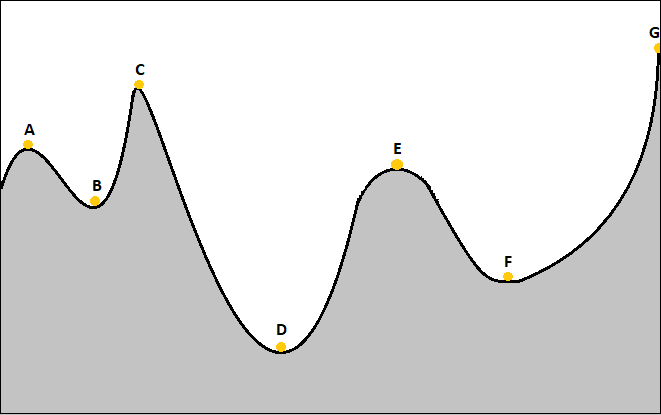
\includegraphics[scale=0.6]{../../../../Screeny/mixmax.png}
		\caption{Przebieg funkcji wraz z zaznaczonymi ekstremami}
		\label{minmax}		
\end{center}	
\end{figure}

Większość metod optymalizacyjnych ma zasięg lokalny, co znaczenie utrudnia poszukiwanie rozwiązania problemu jako, że algorytmy kończą swoje dzialanie w chwili gdy wartość funkcji celu osiągnie wartość ekstremum lokalnego. Powodem tych problemów jest zależność metod optymalizacyjnych od pochodnych funkcji, które to z koleji nie są wystarczająco odporne na nieciągłości czy też rozległe wielomodalności.
\par

\subsection{Podstawowe pojęcia}
W terminologi algorytmów genetycznych używa się następująch pojęć zapożyczonych z genetyki naturalnej \cite{michal}, \cite{maszynowe_sel}:\\

\textbf{Osobnik} - podstawowa jednostka charakteryzująca się pewnym przystosowaniem do środowiska w którym żyje czego miarą jest wartość funkcji celu obliczona dla tego osobnika. Dany osobnik jest wektorem liczb rzeczywistych, potencjalnym rozwiązaniem całego problemu optymalizacji.

\textbf{Populacja} - zbiór osobników ulegający zmianie w kolejnych iteracjach algorytmu jako, że słabsze osobniki są zastępowane przez nowe, lepiej przystosowane.

\textbf{Genotyp} - zbiór informacji przypisany do każdego osobnika indywidualnie, opisujący proponowane rozwiązanie problemu optymalizacyjnego.

\textbf{Fenotyp} - zbiór cech osobnika podlegających ocenie funkcji przystosowania.

\textbf{Chromosom} - jest to uporządkowany ciąg genów, który inaczej nazywany jest łańcuchem. W chromosomie zakodowany jest fenotyp i ewentualnie pewne informacje pomocnicze dla algorytmu genetycznego.

\textbf{Gen} - jest to pojedyńczy element chromosomu.

\textbf{Grupa rozrodcza} - zbiór osobników słóżących jako podstawa do utworzenia osobnika potomnego.

\textbf{Funkcja celu} - funkcja pozwalająca określić miarę przystosowania i jakość konkretnego osobnika z punktu widzenia rozwiązywanego problemu. Jako argument przyjmuje ona wektor będący odpowiednikiem osobnika.

\textbf{Funkcja dopasowania} - jest to funkcja stanowiąca modyfikacje funkcji celu tak aby zachować zależność iż im większa wartość funkcji dopasowania dla danego osobnika tym osobnik jest lepszy.

\textbf{Selekcja} - technika mająca na celu wybór osobników, które przedostaną się do grupy rozrodczej tworzącej potomstwo.

\textbf{Mutacja} - technika mająca na celu utworzenie nowego osobnika na podstawie osobników znajdujących się w grupie rozrodczej .

\textbf{Krzyżowanie} - technika mająca na celu utworzenie nowego osobnika na podstawie osobnika wynikowego mutacji oraz osobnika z aktualnej populacji.

\textbf{Operacje genetyczne} - zbiór operacji takich jak selekcja, mutacja, krzyżowanie.

\subsection{Pseudokod}
\par
 Większość algorytmów optymalizacyjnych stosuje procedure postępowania w której to z każdym krokiem działania algorytmu coraz bardziej zbliżamy się do rozwiązania optymalnego. Algorytmy tego typu zazwyczaj rozpoczynają poszukiwanie startując z konkretnego punktu, a następnie po uwzglednieniu dodatkowych informacji przemieszczają się dalej dochodząc po wielu iteracjach do rozwiązania końcowego.\\
\par
 Podobnie jak w algorytmach ewolucyjnych początkiem działania algorytmu ewolucji różnicowej jest utworzenie pierwszej populacji osobników będących pierwszymi potencjalnymi rozwiązaniami problemu. W każdej iteracji osobniki są poddawane ocenie zgodnie z przyjętą odgórnie funkcją celu. W kontekście algorytmu ewolucji różnicowej, osobnik zdefiniowany jest jako n-elementowy wektor liczb rzeczywistych będący permutacją n-elementowego zbioru:\\
$$
 \overrightarrow{x_{i}}=\{x_{i,1},x_{i,2},...x_{i,n}\}, j = 1,2,...,n
$$
Natomiast populacje można określić jako:\\
$$
X=\{\overrightarrow{x_{1}},\overrightarrow{x_{2}},...\overrightarrow{x_{i}}\}, i = 1,2,...,n
$$
Następnie przeprowadzana jest reprodukcja w wyniku której otrzymujemy grupę rozrodczą. Grupa rozrodcza stanowi podstawę do przeprowadzenia operacji genetycznych jakimi są mutacja oraz krzyżowanie. Operacja mutacji dokonuje przekształceń genetycznych na danej grupie rozrodczej, w wyniku których powstaje nowy osobnik. Poddawany jest on operacji krzyżowania. Dopiero wynik tych dwóch operacji daje rezultat w postaci osobnika potomnego, którego współczynnik przystosowania zostaje oceniony. W sytuacji gdy będzie on większy od współczynnika przystosowania osobnika z obecnej populacji, nastąpi ich podmiana, a więc osobnik potomny zajmie w populacji miejsce poprzednika. Warunkiem zakończenia algorytmu może być na przykład brak zmienności wyniku w kolejnych n iteracjach, bądź też osiągnięcie zadawalającego poziomu przystosowania.\\
\par
Opisane powyżej zależności można w ogólności zaprezentować w postaci pseudokodu algorytmu przedstawionego na \ref{algo}.

\begin{figure}[h!]
\begin{center}
		\includegraphics[scale=1]{../../../../Screeny/algofinal.png}
		\caption{Schemat algorytmu ewolucyjnego}
		\label{algo}		
\end{center}	
\end{figure}

Na schemacie \ref{algo} zauważalna staje się odmienność algorytmu ewolucji różnicowej od klasycznych algorytmów ewolucyjnych głównie w kontekście sposobu dokonywania operacji mutacji.
Dobór metod selekcji, mutacji czy też krzyżowania nie może zostać jednoznacznie określony i być uniwersalny dla wszystkich problemów, które ma on rozwiązywać. Poprawność i jakość działania metod jest ściśle zależna od charakteru rozwiązywanego problemu. Z tego również względu w niektórych przypadkach konieczne jest dokonanie zmian w klasycznym algorytmie ewolucyjnym, w wyniku czego mamy doczynienia ze zmodyfikowanym algorytmem ewolucji różnicowej.
%---------------------------------------------------------------------------

\section{Opis kwadratowego zagadnienia przydziału}\label{sec:strukturaDokumentu}

Kwadratowe zagadnienie przydziału jest jednym z fundamentalnych problemów optymalizacyjnych zajmujących się problemami rozlokowania obiektów. Problem należy do klasy problemów NP-trudnych co oznacza, że nie ma znanego i jednoznacznie określonego algorytmu rozwiązującego ten typ problemu w stosunkowo krótkim czasie. Sprawdzenie wszystkich opcji w celu znalezienia rozwiązania najlepszego nawet małego rozmiaru problemu okazuje się być probematyczne i długotrwałe.\\
\par
\textbf{Model matematyczny kwadratowego zagadnienia przydziału}\\
\par
Dany jest zbiór n budynków oraz z zbiór n lokalizacji. Pomiędzy każdymi dwoma lokalizacjami znana jest odległość oraz wartość przepływu. Wartość przepływu można interpretować jako koszt transportu dóbr pomiędzy dwiema lokalizacjami. Celem zadania jest takie przypisanie budynków do danych lokalizacji by zminimalizować sume odległości pomiędzy każdymi dwoma budynkami pomnożoną przez odpowiadającą danej trasie wartość przepływu.

Formalna definicja kwadratowego zagadnienia przydziału jest następująca \cite{chmiel} :

Dane są dwie rzeczywiste macierze F = ($f_{ij}$) oraz D = ($d_{ij}$) o wymiarze$ n \times n $każda, gdzie odpowiednio:\\
$f_{ij}$ - macierz przepływu pomiędzy punktami i oraz j,
$d_{ij}$ - macierz odległości, określająca odległość pomiędzy punktami i oraz j,
$$
\sum_{i=1}^{n}\sum_{j=1}^{n}f_{ij} \cdot d_{ij} \longrightarrow min
$$
Należy zaznaczyć również fakt iż jeden budynek może zostać przypisany do jednej lokalizacji oraz do jednaj lokalizacji może zostać  przypisany tylko jeden budynek. Poniżej zamieszczono rysunek obrazujący kwadratowe zagadnienie przydziału.

\begin{figure}[h!]
\begin{center}
		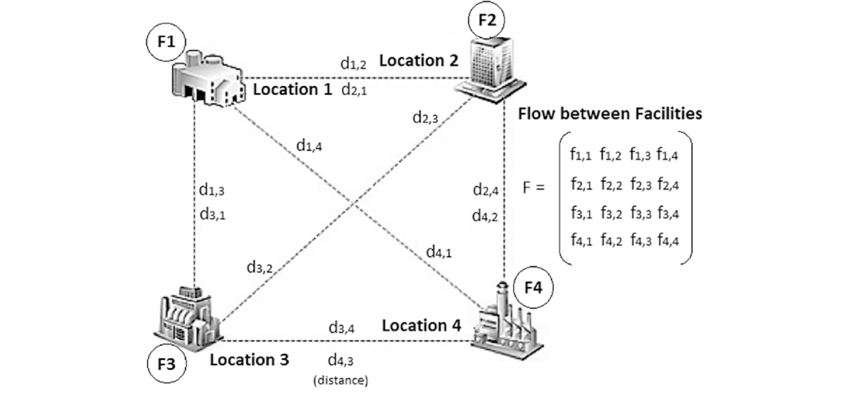
\includegraphics[scale=0.5]{../../../../Screeny/qap.png}
		\caption{Przedstawienie kwadratowego zagadnienia przydziału \cite{qap_rys}}
		\label{qap}		
\end{center}	
\end{figure}


\chapter{Metody selekcji}\label{metody_selekcji}

Jednym z etapów algorytmu ewolucyjnego jest selekcja polegająca na wyborze osobników, które przedostaną się do grupy rozrodczej tworzącej potomstwo. Znanych jest kilka metod selekcji na podstawie których dokonuje się wyboru osobników z różnym prawdopodobieństwem. Metody te w większości zostały opracowane w taki sposób by dawały większe szanse przetrwania osobnikom lepiej do tego przystosowanym, a więc osobnikom o większym współczynniku funkcji przystosowania. 

Metody selekcji zostały zaimplementowane w dwojaki sposób. Pierwszym z nich jest możliwość pojawienia się danego osobnika w grupie rodzicielskiej wiecej niż jeden raz. Druga technika nakazuje różnorodność osobników w obrębie danej instancji grupy. Poniżej przestawiono idee metod selekcji podlegających rozważaniom w ramach tej pracy. Zgodnie z przyjętymi założeniami do grupy rozrodczej przedostają się 3 osobniki z populacji rodziców, co sprowadza się do faktu iż wybór należy powtórzyć trzykrotnie. Implementacje metod powstały w oparciu o \cite{maszynowe_sel}, \cite{gracjan}.

%---------------------------------------------------------------------------

\section{Losowy wybór}\label{sec:strukturaDokumentu}

Z populacji wybierany jest osobnik przechodzący do grupy rozrodczej w oparciu o  wylosowaną liczbę odpowiadającą indeksowi konkretnego osobnika. Metoda ta jest niezależna od wartości funkcji przystosowania, a więc daje równe szanse każdemu z osobników. Prawdopodobieństwo wylosowania danego osobnika, z populacji składającej się z n osobników,jest równe :
\vspace{0,4cm}
$$
P = \frac{1}{n}
$$

\par
Odpowiadająca funkcja w programie :\textbf{ RandomWitoutRestrictions()}

\begin{program}
\begin{lstlisting}[
 basicstyle=\scriptsize,]
        public List<int> RandomWitoutRestrictions()
        {
            List<int> WhichIndividuals = new List<int>();
            int number = 3;
            var rand = new System.Random();

            while (number != 0)
            {
                WhichIndividuals.Add(Kit.GiveRandomNumber(WhichIndividuals, Population.Count - 1, rand));
                number--;
            }
            return WhichIndividuals;
        }
\end{lstlisting}
\end{program}

%---------------------------------------------------------------------------

\section{Metoda rankingowa}\label{sec:kompilacja}


W metodzie selekcji rankingowej dla osobników składających się na populacje rodziców obliczana jest wartość funkcji celu, na której to podstawie tworzony jest ranking. Osobniki z najmniejszą wartością wyniku uzyskują najwyższe miejsca w rankingu \cite{selekcje}. Miejsce w rankingu jest argumentem funkcji na podstawie której obliczane jest prawdopodobieństwo wyboru danego osobnika jako rodzica. Rodzic zostanie poddany kolejnym operacjom (mutacja, krzyżowanie).\\
 Funkcja stosowana na której to podstawie tworzony jest ranking może być funkcją liniową. Wówczas osobniki zajmujące w rankingu będącym N elementowym wektorem konkretne miejsce określone rangą, gdzie N to ilość osobników w populacji otrzymują prawdopodobieństwo przejścia do grupy rodzicielskiej określone poniższą zależnością \cite{Lam92}:
$$
P = \frac{ranga}{\sum_{j=1}^{n}j}
$$

\begin{table}[h!]
\begin{center}
\begin{tabular}{|c|c|c|c|}
\hline
\textbf{Osobnik}  & \textbf{Funkcja celu} & \textbf{Ranga} & \textbf{Prawdopodobieństwo}\\
\hline
Osobnik 1 & 373 & 1 & 6,(6) \% \\
\hline
Osobnik 2 &254 & 2  & 13,(3)  \% \\
\hline
Osobnik 3 & 202 & 3 & 20  \% \\
\hline
Osobnik 4 & 136 & 4 & 26,(6)  \% \\
\hline
Osobnik 5 & 10 & 5 & 33,(3)  \% \\
\hline
\end{tabular}
\caption{Wartości parametrów na kolejnych osobników w metodzie rankingowej}
\end{center}
\end{table}

\vspace{0,4cm}

\begin{figure}[h]
		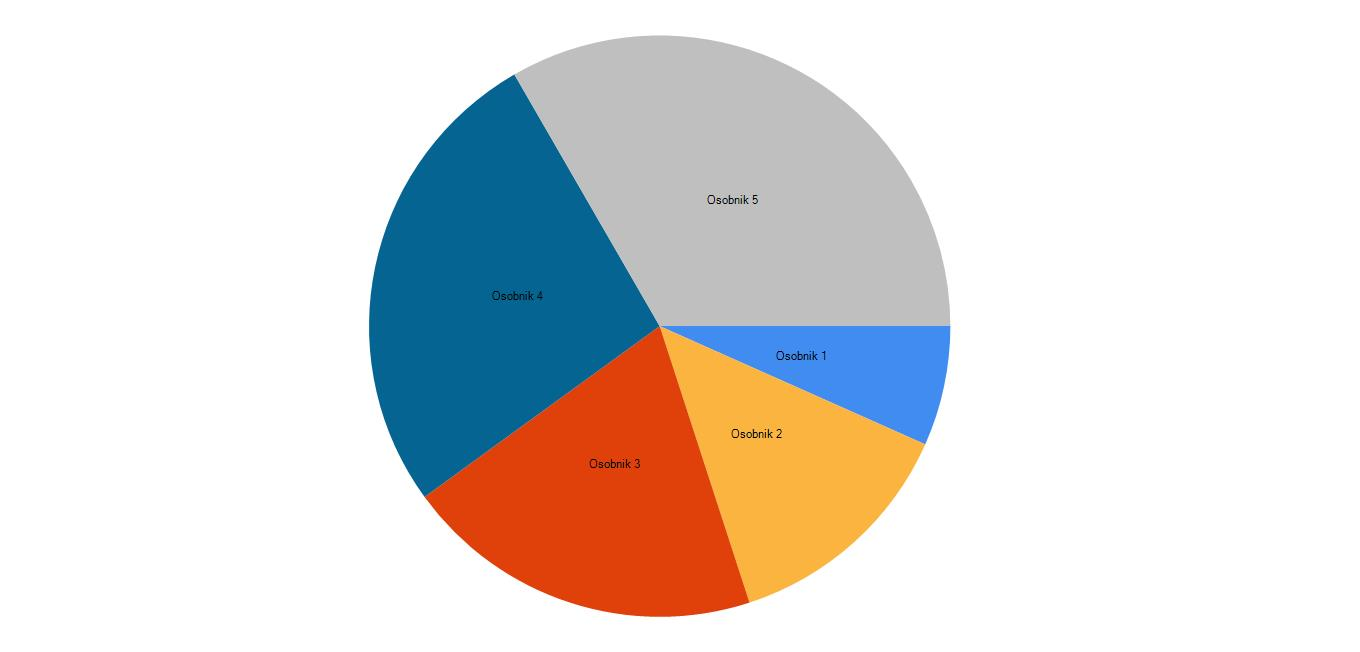
\includegraphics[scale=0.45]{../../../../Screeny/metoda_rankingowa.jpg}
		\caption{Rozkład prawdopodobieństwa w metodzie rankingowej}
		\label{ranking}			
\end{figure}
\par
Na podstawie \ref{ranking} zauważalny staje się fakt, iż rozkład prawdopodobieństwa nie jest bezpośrednio zależny od wartości funkcji celu. W metodzie tej zwiększone są więc szanse przejścia do grupy rodzicielskiej osobników z małą wartością funkcji dopasowania, które to miałyby małe szanse przejścia dalej w metodzie selekcji zależnej od wartości funkcji celu. Metoda może wydawać się niekorzystna z punktu widzenia osobników z dużą wartością funkcji dopasowania jako, że mogą otrzymać one niewiele większe prawdopodobieństwo przejścia do grupy rodzicielskiej od osobników znajdujących się range niżej pomimo iż ich wartości funkcji celu mogą różnić się znacząco.
\par
\vspace{0,4cm}
Odpowiadająca funkcja w programie : \textbf{RankingMethod()}
\begin{program}
\begin{lstlisting}[
 basicstyle=\scriptsize,]
        public List<int> RankingMethond()
        {
            List<int> WhichIndividuals = new List<int>();
            List<int> WhichIndividualsIndex = new List<int>();
            List<int> WhichIndividualBeforeSelection = new List<int>();
            List<int> ResultsOfObjectiveFunction = inputdata.ObjectiveFunctionVector(Population);

            var rand = new System.Random();
            int size_tmp = size;
            int number = 3;

            while (size_tmp != 0)
            {
                var index = ResultsOfObjectiveFunction.IndexOf(ResultsOfObjectiveFunction.Min());
                ResultsOfObjectiveFunction[index] = Int32.MaxValue;

                int numberOfIter = size_tmp;
                while (numberOfIter != 0)
                {
                    WhichIndividualBeforeSelection.Add(index);
                    numberOfIter--;
                }
                size_tmp--;
            }

            while (number != 0)
            {
                var tmp = Kit.GiveRandomNumber(WhichIndividualsIndex, WhichIndividualBeforeSelection.Count - 1, rand);
                for (int i = 0; i < WhichIndividualBeforeSelection.Count; i++) // to w celu uniknięcia powtórzeń w wektorach
                {
                    if (WhichIndividualBeforeSelection[i] == WhichIndividualBeforeSelection[tmp])
                        WhichIndividualsIndex.Add(i);
                }

                WhichIndividuals.Add(WhichIndividualBeforeSelection[tmp]);
                number--;
            }
            return WhichIndividuals;
        }
\end{lstlisting}
\end{program}

%---------------------------------------------------------------------------

\section{Metoda ruletki}\label{sec:narzedzia}


W metodzie ruletki każdemu chromosomowi zostaje przypisany wycinek koła \cite{selekcje}. Im silniejszy osobnik tym większy wycinek koła dostaje, gdyż zależność wartości funkcji przystosowania i prawdopodobieństwo wylosowania osobnika jest wprost proporcjonalna. Każdy osobnik tworzący populacje poddawany jest ocenie funkcji celu. Maksymalna wartość funkcji przystosowania oznacza najmniejszą wartość funkcji celu. Uzyskana wartość funkcji przystosowania w stosunku do sum wartości tej funkcji wszystkich osobników populacji wyznacza prawdopodobieństwo wylosowania danego osobnika na rodzica. Prawdopodobieństwo wylosowania danego osobnika dane jest następującą zależnością:
$$
P_i = \frac{f(i)}{\sum_{j=1}^{n}f(j)}
$$
Gdzie f(x) - funkcja przystosowania\\
\par
Funkcją przystosowania w rozważanym poniżej przypadku jest funkcja przyporządkowującą największej wartości funkcji celu wartość najmniejszą, a wartości najmniejszej wartość największą.

\begin{table}[h!]
\begin{center}
\begin{tabular}{|c|c|c|c|}
\hline
\textbf{Osobnik}  & \textbf{Funkcja celu} & \textbf{Funkcja dopasowania} & \textbf{Prawdopodobieństwo}\\
\hline
Osobnik 1 & 373 & 10 & 1,02  \% \\
\hline
Osobnik 2 &254 & 136  & 13,95  \% \\
\hline
Osobnik 3 & 202 & 202 & 20,72  \% \\
\hline
Osobnik 4 & 136 & 254 & 26,05  \% \\
\hline
Osobnik 5 & 10 & 373 & 38,25  \% \\
\hline
\end{tabular}
\caption{Wartości parametrów na kolejnych osobników w metodzie ruletki}
\end{center}
\end{table}

\vspace{0,4cm}

\begin{figure}[h]
		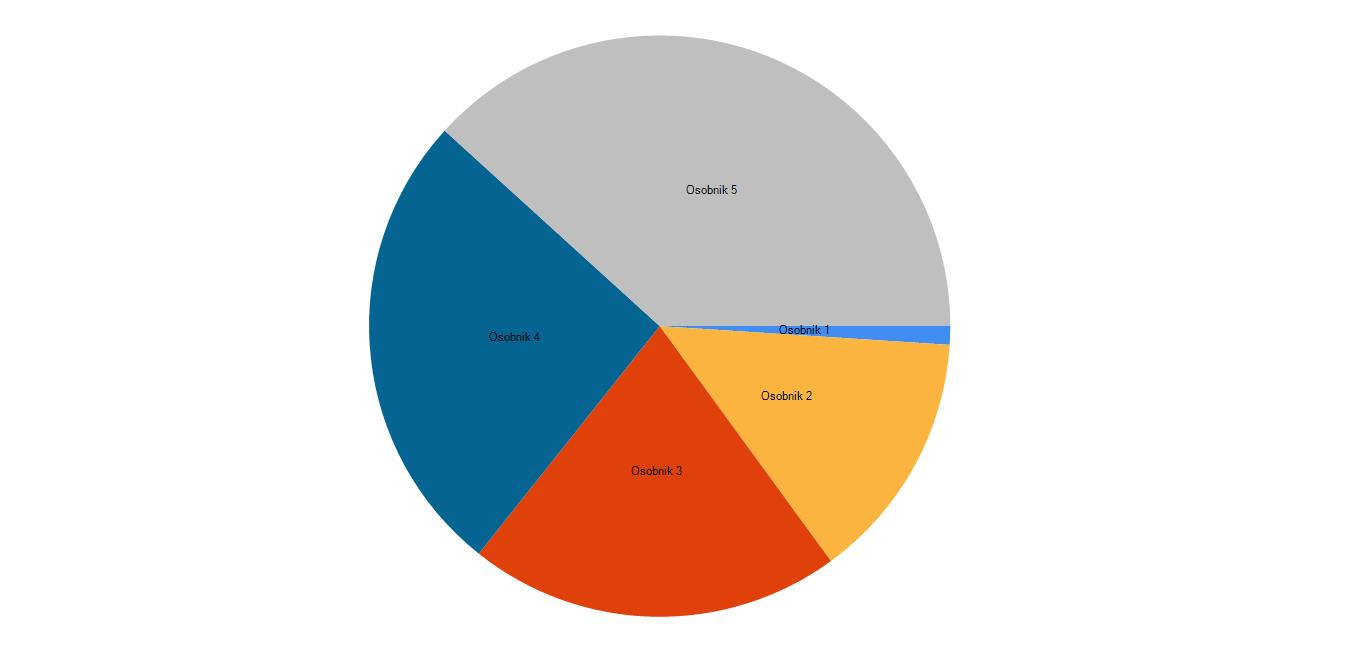
\includegraphics[scale=0.45]{../../../../Screeny/metoda_ruletki.jpg}
		\caption{Rozkład prawdopodobieństwa w metodzie ruletki}
		\label{ruletka}			
\end{figure}
\par
W metodzie ruletki wkład każdego osobnika w rozkład prawdopodobieństwa jest wprost proporcjonalny do wartości jego funkcji dopasowania. Wady tej metody stają się widoczne, w sytuacji gdy dany osobnik zajmuje większość powierzchni koła, gdyż osobniki o małej wartości funkcji dopasowania są przedwcześnie eliminowane, a więc nie mają wielkiej szansy by zostać wylosowane. Prowadzi to do braku różnorodności w kolejnych grupach rozrodczych, co utrudnia dojście do lepszego wyniku. Z problemem tym dobrze sobie radzi wspomniana wyżej metoda rankingowa gzdei eliminowana jest możliwość dużej przewagi jednego z nich nad resztą.\\
\par
Odpowiadająca funkcja w programie : \textbf{RouletteMethod()}

\begin{program}
\begin{lstlisting}[
 basicstyle=\scriptsize,]
        public List<int> RouletteMethond()
        {
            List<int> WhichIndividuals = new List<int>();
            List<int> ResultsOfObjectiveFunction = inputdata.ObjectiveFunctionVector(Population);
            List<Tuple<int, int>> tuple = new List<Tuple<int, int>>();
            int range_begin = 0;
            int range_end = 0;
            var rand = new System.Random();
            int number = 3;

            foreach (var elem in ResultsOfObjectiveFunction)
            {
                range_end += elem;
                tuple.Add(new Tuple<int, int>(range_begin, range_end));
                range_begin = elem + 1;
            }

            while (number != 0)
            {
                var tmp = Kit.GiveRandomNumber(WhichIndividuals, ResultsOfObjectiveFunction.Sum(), rand);
                for (int i = 0; i < tuple.Count; i++)
                {
                    if (tuple[i].Item2 > tmp)
                    {
                        WhichIndividuals.Add(i);
                        number--;
                        break;
                    }
                }
            }
            return WhichIndividuals;
        }
\end{lstlisting}
\end{program}

%---------------------------------------------------------------------------

\section{Metoda turniejowa}\label{sec:narzedzia}


Metoda selekcji turniejowej polega na rozgrywaniu turnieju pomiędzy osobnikami tworzącymi populacje. W wyniku jednorazowej rozgrywki wygrywa osobnik o większej wartości funkcji przystosowania, przechodząc tym samym do kolejnej rundy. W każdym turnieju zwycięża jeden osobnik, którego to genotyp jest wykorzystywany przy kolejnych operacjach genetycznych. Populacja dzielona jest na dwuosobnikowe podgrupy w których to dokonywane są rozgrywki. W przypadku nieparzystego rozmiaru populacji, osobnik ostatni przechodzi do kolejnej rundy bezkonkurencyjnie. \\
\par
Metoda turniejowa nie wymaga znajomości optymalizowanej funkcji, konieczny jest jedynie informacja o relacji zachodzącej pomiędzy dwoma kolejnymi osobnikami. 
\par
Odpowiadająca funkcja w programie : \textbf{TournamentMethod()}

\begin{program}
\begin{lstlisting}[
 basicstyle=\scriptsize,]
 public List<int> TournamentMethond()
        {
            List<int> WhichIndividuals = new List<int>();
            List<int> ResultsOfObjectiveFunction = inputdata.ObjectiveFunctionVector(Population);
            List<int> ResultsOfObjectiveFunction_const = new List<int>();
            ResultsOfObjectiveFunction_const.AddRange(ResultsOfObjectiveFunction);
            List<int> TournamentTable = new List<int>();
            int number = 3;

            while (number != 0)
            {
                int sizeOfTournament_const = ResultsOfObjectiveFunction.Count;
                while (sizeOfTournament_const > 1)
                {
                    for (int i = 0; i < sizeOfTournament_const; i++)
                    {
                        TournamentTable.Add(Math.Min(ResultsOfObjectiveFunction[i], ResultsOfObjectiveFunction[i + 1]));
                        i++;

                        if ((sizeOfTournament_const \% 2) == 1 \&\& i == sizeOfTournament_const - 2)
                        {
                            TournamentTable.Add(ResultsOfObjectiveFunction.Last());
                            i++;
                        }
                    }

                    if (TournamentTable.Count == 1)
                        break;
                    sizeOfTournament_const = TournamentTable.Count;
                    ResultsOfObjectiveFunction.RemoveAll(elem => ResultsOfObjectiveFunction.Contains(elem));
                    ResultsOfObjectiveFunction.AddRange(TournamentTable);
                    TournamentTable.RemoveAll(elem => TournamentTable.Contains(elem));
                }

                var index = ResultsOfObjectiveFunction_const.FindIndex(value => value == TournamentTable[0]);
                WhichIndividuals.Add(index);
                ResultsOfObjectiveFunction_const[index] = Int32.MaxValue;
                ResultsOfObjectiveFunction.RemoveAll(elem => ResultsOfObjectiveFunction.Contains(elem));
                ResultsOfObjectiveFunction.AddRange(ResultsOfObjectiveFunction_const);
                TournamentTable.RemoveAt(0);
                number--;
            }
            return WhichIndividuals;
        }
\end{lstlisting}
\end{program}

%---------------------------------------------------------------------------

\section{Metoda elitarna}\label{sec:przygotowanieDokumentu}

W metodzie tej nacisk położony jest na to, aby do grupy rozrodczej przedostały się z prawdopodobieństwem równym p=100\% osobniki najlepiej przystosowane. W poprzednich metodach(ruletki, turniejowa, rankingowa) prawdopodobieństwo przejścia do grupy rozrodczej dla osobników z większym wskaźnikiem funkcji przystosowania jest jedynie większe niż dla pozostałych osobników. Nie ma jednak gwarancji przedostania się dalej osobników najlepiej przystosowanych. W strategii elitarnej do grupy na której zostanie dokonana operacja mutacji a następnie krzyżowania przedostaje się n osobników z populacji odznaczających się najwyższym wskaźnikiem funkcji przystosowania \cite{GPS}.\\
\par
Zastosowanie elitaryzmu jako metody selekcji daje pewność iż do grupy rodzicielskiej przedostaną się najlepiej do tego przystosowane osobniki. Dzięki temu unika sie sytuacji w której stosunkowo mocny osobnik w wyniku operacji genetycznych zostanie osłabiony a co za tym idzie, nie przechodzi on do grupy rodzicielskiej.\\
\par
Odpowiadająca funkcja w programie : \textbf{ElitistMethod()}

\begin{program}
\begin{lstlisting}[
 basicstyle=\scriptsize,]
        public List<int> ElitistMethond()
        {
            List<int> WhichIndividuals = new List<int>();
            List<int> ResultsOfObjectiveFunction = inputdata.ObjectiveFunctionVector(Population);
            int number = 3;

            while (number != 0)
            {
                int index = ResultsOfObjectiveFunction.FindIndex(min => min == ResultsOfObjectiveFunction.Min());
                WhichIndividuals.Add(index);
                ResultsOfObjectiveFunction[index] = Int32.MaxValue;
                number--;
            }

            return WhichIndividuals;
        }
\end{lstlisting}
\end{program}


\chapter{Operacja mutacji}\label{cha:pierwszyDokument}

Mutacja stanowi najważniejszą część algorytmu ewolucyjnego, z tego względu stosuje się wiele modyfikacji w celu rozwoju i poprawy działania tego operatora.
Mutacja stosowana w algorytmie ewolucji różnicowej zdefiniowana jest w odmienny sposób w stosunku do algorytmu ewolucyjnego w którym to genotyp stanowią wartości binarne, a operator mutacji ma za zadanie wprowadzenie zmian na zasadzie negacji obecnej wartości genu. W mutacji różnicowej zastosowana jest operacja odejmowania od siebie dwóch wektorów tworząc tym samym wektor różnicowy, czemu również algorytm zawdzięcza swoją nazwe z ang. \textsl{difference} \cite{przystojny_koles}. Wktor różnicowy jest zatem miarą określającą odległość pomiędzy dwoma osobnikami.  Podobnie jak ma to miejsce w innych algorytmach należących do grona algorytmów ewolucyjnych, tak i ewolucja różnicowa posiada wiele alternatywnych metod mutacji. Metody mutacji różnicowej różnią się od siebie głównie elementami takimi jak:

\begin{enumerate}
\item Sposób  wyboru osobnika będącego wektorem bazowym, a więc wektorem znajdującym się w grupie rozrodczej lecz nie wchodzącym w skład wektora różnicowego \textsl{X},
\item Liczba wektorów różnicowych \textsl{Y}
\end{enumerate}
\par
W związku z powyższym, metody mutacji mogą przyjąć następującą nomenklature \textsl{DE/X/Y/Z}. \textsl{Z} oznacza rodzaj zastosowanego operatora krzyżowania w związku z czym parametr ten nie będzie uwzględniony w poniższym opisie metod mutacji . Wybór danej metody jest zależny od specyfiki rozwiązywanego problemu i dla różnych jego instancji może dawać odmienne rezultaty. Ogólny wzór opisujący sposób powstawania genu osobnika potomnego można wyrazić następująco:
$$
 \forall U_{i} =S_{r_{1}i} + \sum_{j=1}^{n} F_{j} \cdot (S_{r_{2j}i} - S_{r_{3j}i})
$$
Gdzie:\\
$j$ - liczba wektorów różnicowych,\\
$U_{i}$ - i-ty gen osobnika potomnego,\\
$r_{1}$,$ r_{2}$,$ r_{3}$ - osobniki wchodzące w skład populacji,\\
$S_{r_{1}i}$ - i-ty gen osobnika $r_{1}$\\
$F$ - współczynnik mutacji, $F \in (0,1)$,\\
$S$ -populacja\\


Wprowadzono zależność iż osobnikami biorącymi udział w procesie mutacji są osobniki uprzednio wybrane poprzez metodę selekcji \cite{diff2}. W implementacji metod mutacji dodatkowo należało zastosować pewnego rodzaju modyfikacje, wynikającą z faktu iż pojedyńczy osobnik jest ciągiem będącym permutacją, a więc nie dopuszcza istnienia wartości zmiennoprzecinkowych. Jako że wektor różnicowy mnożony jest przez współczynnik mutacji będący wartością zmiennoprzecinkową końcowy gen również jest wartością zmiennoprzecinkową. W celu eliminacji takiej sytuacji, należało dokonać stosownego rodzaju skalowanie uwzględniające relacje mniejszości i większości pomiędzy poszczególnymi genami, a jednocześnie zamieniające wartości zmiennoprzecinkowe na całkowite. Implementacje wspomnianej modyfikacji zamieszczono poniżej:

\begin{program}[h!]
\begin{lstlisting}[
 basicstyle=\scriptsize,]
	public void Normalize(List<double> MutatedIndividual_tmp, List<int> MutatedIndividual)
        {
            List<double> ListToConvert = MutatedIndividual_tmp;
            int cnt = 1;

            while (cnt != (MutatedIndividual_tmp.Count + 1))
            {
                var index = ListToConvert.FindIndex(min => min == MutatedIndividual_tmp.Min());
                MutatedIndividual[index] = cnt;
                MutatedIndividual_tmp[index] = Double.MaxValue;//.RemoveAt(MutatedIndividual_tmp.FindIndex(min => min == MutatedIndividual_tmp.Min()));

                cnt++;
            }
        }
\end{lstlisting}
\end{program}

 Poniżej zestawione zostały strategie najczęściej spotykane w literaturze i opisane szczegółowo w \cite{doktorat}.
%---------------------------------------------------------------------------

\section{Klasyczna mutacja: DE/rand/1}\label{sec:strukturaDokumentu}

Podstawową strategią  stosowaną jako operator mutacji jest strategia zakładająca uznanie za wektor bazowy pierwszego osobnika znajdującego się w grupie rozrodczej \cite{diff2}. Jako, że grupa rozrodcza składa się z trzech osobników, dwa pozostałe są odpowiedzialne za utworzenie wektora różnicowego, który jest następnie skalowany współczynnikiem $F = 0,8$. Przyjęta wartość jest najczęściej spotykaną w literaturze wartością czynnika skalującego, analiza wpływu tego marametru na działanie metod mutacji zostanie przedstawiona w dalszej częsi pracy. Powyżej wspomniane zależności można opisać wzorem:
$$
 \forall U_{i} =S_{r_{1}i} + F \cdot (S_{r_{2}i} - S_{r_{3}i})
$$
Poniżej zaprezentowano implementacje metody wraz z uwzględnieniem konieczności normalizacji wektora będącego wynikiem mutacji danej powyższym wzorem. 

\begin{program}[h!]
\begin{lstlisting}[
 basicstyle=\scriptsize,]
        public List<int> ToMutate()
        {
            List<int> MutatedIndividual = new List<int>(new int[Population.Count]);
            List<double> MutatedIndividual_tmp = new List<double>();
            List<int> Randoms = RandomWitoutRestrictions();
            double DefaultValueForMut = 0.8;

            for (int j = 0; j < Population.Count; j++)
            {
                double value = Population[Randoms[0]][j] + DefaultValueForMut * (Population[Randoms[1]][j] - Population[Randoms[2]][j]);
                MutatedIndividual_tmp.Add(value);
            }

            Normalize(MutatedIndividual_tmp, MutatedIndividual);
            return MutatedIndividual;
        }
\end{lstlisting}
\end{program}

%---------------------------------------------------------------------------
\section{Modyfikacje metod mutacji}\label{sec:kompilacja}

Klasyczna metoda mutacji pomimo częstego jej stosowania, nie zawsze daje oczekiwane rezultaty.  W pewnych instancjach problemów efektywniejszym działaniem mogą wykazać się metody mutacji do których zostały wprowadzone pewnego rodzaju modyfikacje. Poniżej zestawionych zostało kilka możliwych modyfikacji opisanych bardziej szczegółowo \cite{diff2}.

\subsection{Strategia II: DE/best/1}\label{sec:kompilacja}

W strategii II miejsce wektora bazowego zajmuje wektor odznaczający się zajwiekszą wartością funkcji celu, a więc wektor najlepszy. W celu znalezienia najlepszego osobnika konieczne jest przeszukanie całej populacji, co może okazać się niekorzystne w kontekście złożoności obliczeniowej i eksploatacji algorytmu. Wektor różnicowy jest różnicą dwóch losowo wybranych osobników przeskalowanych współczynnikiem mutacji. Zależność strategii DE/best/1 można opisać wzorem:
$$
 \forall U_{i} =S_{best,i} + F \cdot (S_{r_{1}i} - S_{r_{2}i})
$$
Poniżej zaprezentowano implementacje metody wraz z uwzględnieniem konieczności normalizacji wektora będącego wynikiem mutacji danej powyższym wzorem. 

\begin{program}[h!]
\begin{lstlisting}[
 basicstyle=\scriptsize,]
        public List<int> ToMutate2()
        {
            List<int> MutatedIndividual = new List<int>(new int[Population.Count]);
            List<double> MutatedIndividual_tmp = new List<double>();

            List<int> Best = ElitistMethond(1);
            List<int> Difference = RandomWitoutRestrictions(2);

            double DefaultValueForMut = 0.8;

            for (int j = 0; j < Population.Count; j++)
            {
                double value = Population[Best[0]][j] + DefaultValueForMut * (Population[Difference[0]][j] - Population[Difference[1]][j]);
                MutatedIndividual_tmp.Add(value);
            }

            Normalize(MutatedIndividual_tmp, MutatedIndividual);
            return MutatedIndividual;
        }
\end{lstlisting}
\end{program}

%---------------------------------------------------------------------------

\subsection{Strategia III: DE/rand/$n_{v}$}\label{sec:narzedzia}

Strategię III od poprzednich metod wyróżnia fakt iż nowy osobnik powstaje w oparciu o sume wektorów różnicowych a nie na podstawie jednego wektora różnicowego tak jak miało to miejsce w przypadku poprzednich metod. Istnieje więc dodatkowy parametr $n_{v}$ określający ilość wektorów różnicowych. W sytuacji gdy $  2 * n_{v} + 1$ jest większe od rozmiaru populacji \textsl{n}, do $n_{v}$ zostaje przypisana defaultowa wartość równa największej liczbie wektorów różnicowych które można utworzyć przy danym rozmiarze populacji \textsl{n}\\
$$
 n_{v} = (n - 1) / 2
$$

Wartość będąca sumą wektorów różnicowych jest następnie skalowana współczynnikiem mutacji \textsl{F}. Opisane powyżej zależności można zapisać w postaci wzoru:\\
$$
 \forall U_{i} =S_{r_{1}i} +  F \cdot \sum_{k=1}^{n_{v}}(S_{r_{2}i} - S_{r_{3}i})
$$
Strategie III można wyrazić za pomocą poniższej implementacji.

\begin{program}[h!]
\begin{lstlisting}[
 basicstyle=\scriptsize,]
public List<int> ToMutate3(int number_of_vectors)
        {
            List<int> MutatedIndividual = new List<int>(new int[Population.Count]);
            List<double> MutatedIndividual_tmp = new List<double>();
            int n = 2 * number_of_vectors + 1;

            if (n > Population.Count)
            {
                number_of_vectors = (Population.Count - 1) / 2;
            }

            List<int> Randoms = RandomWitoutRestrictions(3);
            double DefaultValueForMut = 0.8;
            for (int j = 0; j < Population.Count; j++)
            {
                int difference = 0;
                int number = number_of_vectors;
                while (number != 0)
                {
                    difference += (Population[Randoms[1]][j] - Population[Randoms[2]][j]);
                    number--;
                }

                double value = Population[Randoms[0]][j] + DefaultValueForMut * difference;
                MutatedIndividual_tmp.Add(value);
            }
            Normalize(MutatedIndividual_tmp, MutatedIndividual);
            return MutatedIndividual;
        }
\end{lstlisting}
\end{program}

%---------------------------------------------------------------------------

\subsection{Strategia IV: DE/current to best/$n_{v} +1$}\label{sec:narzedzia}


Strategia ta zawiera w sobie pewne elementy zawarte we wcześniej opisanch metodach mutacji różnicowej. Na osobnika potomnego składa się  $n_{v}$ wektorów różnicowych, będących różnicą dwóch losowo wybranych osobników z populacji, pomnożonych razy współczynnik mutacji (strategia III). Sumuje się także wartość, przemnożonego przez współczynnik mutacji, odrębnego wektora różnicowego w skład którego wchodzi osobnik odznaczajacy się największym współczynnikiem funkcji celu (strategia II) oraz osobnik losowy. Dodatkowo należy również uwzględnić wartość osobnika o indeksie odpowiadającym iteracji w której znajduje się obecnie algorytm. Zależności te opisuje poniższy wzór:\\

$$
 \forall U_{i} = S_{r_{itert}i} +  F \cdot (S_{r_{best}i} - S_{r_{1}i}) +  F \cdot \sum_{k=1}^{n_{v}}(S_{r_{2}i} - S_{r_{3}i})
$$
Implementacje funkcji można określić w następujący sposób:
\begin{program}[h!]
\begin{lstlisting}[
 basicstyle=\scriptsize,]
public List<int> ToMutate4(int number_of_vectors, int iter)
        {
            List<int> MutatedIndividual = new List<int>(new int[Population.Count]);
            List<double> MutatedIndividual_tmp = new List<double>();
            int n = 2 * number_of_vectors + 1;

            if (n > Population.Count)
            {
                number_of_vectors = (Population.Count - 1) / 2;
            }

            List<int> Best = ElitistMethond(1);
            List<int> Randoms = RandomWitoutRestrictions(3);
            double DefaultValueForMut = 0.8;
            for (int j = 0; j < Population.Count; j++)
            {
                int difference = 0;
                int number = number_of_vectors;
                while (number != 0)
                {
                    difference += (Population[Randoms[1]][j] - Population[Randoms[2]][j]);
                    number--;
                }

                double value = Population[iter][j] + DefaultValueForMut * (Population[Best[0]][j] - Population[Randoms[0]][j]) + DefaultValueForMut * difference;
                MutatedIndividual_tmp.Add(value);
            }
            Normalize(MutatedIndividual_tmp, MutatedIndividual);
            return MutatedIndividual;
        }
\end{lstlisting}
\end{program}

%---------------------------------------------------------------------------

\subsection{Mutacja z wprowadzeniem parametru $\leftthreetimes$} \label{sec:narzedzia}

W literaturze \cite{czynnik} można także znaleźć wersje metod mutacji w których wprowadza się modyfikacje powyżej zaprezentowanych metod poprzez wprowadzenie czynnika skalującego $\leftthreetimes$. Parametr ten wprowadza w algorytmie dodatkową losowość, co może wpłynąć korzystnie na szybkość dochodzenia algorytmu do rozwiązania końcowego. Zmiany, w stosunku do poprzednich wersji, dotyczą pomnożenia wektora bazowego przez czynnik skalujący $\leftthreetimes$, gdzie $\leftthreetimes \in (0,1)$. W poprzednich strategiach niezależnie od ich rodzajów wektor bazowy był zawsze wartością nieprzeskalowaną. Można to opisać poniższymi zależnościami:\\

\begin{enumerate}
\item Strategia I : $ \forall U_{i} = \leftthreetimes \cdot S_{r_{1}i} + F \cdot (S_{r_{2}i} - S_{r_{3}i})$
\item Strategia II : $ \forall U_{i} = \leftthreetimes \cdot  S_{best,i} + F \cdot (S_{r_{1}i} - S_{r_{2}i}) $
\item Strategia III : $ \forall U_{i} = \leftthreetimes \cdot  S_{r_{1}i} +  F \cdot \sum_{k=1}^{n_{v}}(S_{r_{2}i} - S_{r_{3}i}) $
\item Strategia IV : $ \forall U_{i} = \leftthreetimes \cdot S_{r_{itert}i} +  F \cdot (S_{r_{best}i} - S_{r_{1}i}) +  F \cdot \sum_{k=1}^{n_{v}}(S_{r_{2}i} - S_{r_{3}i}) $
\end{enumerate}
\par

%---------------------------------------------------------------------------

\section{Dostrajanie parametrów mutacji}\label{sec:kompilacja}

W literaturze \cite{przystojny_koles}, \cite{czynnik}, za wartość parametru mutacji $F$, który to odpowiada za przeskalowanie wektora różnicowego, najczęściej przyjmuje się wartość $F$ = 0.8. Nie mniej jednak jest to wartość uzyskana doświadczalnie, co oznacza iż daje ona najlepsze efekty w większości przypadków testowych. Należy jednak pamiętać o fakcie iż przypadkami testowymi są zazwyczaj standardowe funkcje, a więc w sytuacji gdy mamy doczynienia z bardziej złożonych zagadnieniami wartość $F$ = 0.8 może okazać się nie zadowalająca. Stała wartość parametru $F$ może być więc pewnego rodzaju ograniczeniem. Z tego względu wprowadzenie dynamicznej zmiany tego parametru może okazać się rozwiązaniem poprawiającym działanie algorytmu. Modyfikacja ta sprowadza się do zmiany wartości współczynnika mutacji $F$ w kolejnych iteracjach algorytmu zgodnie z danym wzorem \cite{doktorat}:
$$
F_{t+1} = F_{t} + \frac{(0.5 + F_0)}{g}
$$
\par
Gdzie:\\
$F_{t+1}$ - współczynnik skalującyw kolejnej iteracji,\\
$F{0}$ - współczynnik skalujący w pierwszej iteracji,\\
$g$ - liczba iteracji algorytmu\\
\par
Za początkową wartość parametru $F_{0}$ przyjmue się wartość równą $F_{0}$ = 0.3, w kolejnych iterajach algorytmu wartość ta jest sukcesywnie zwiększana o wartość zależną od założonej początkowo liczby iteracji algorytmu
\par
TODO
Jak coś to można jeszcze zrobic o tym że F jest losowane zgodnie z rozkladem Gaussa



































\include{metody_krzyżowania}
\chapter{Dodatkowe modyfikacje w obrębie algorytmu ewolucji różnicowej}\label{cha:pierwszyDokument}
\section{Sekwencyjny i równoległy algorytm ewolucji różnicowej }
Równoległy opiera się na zastosowaniu 3 populacji osobników o jednakowej liczności. W każdej iteracji, na podstawie populacji rodziców tworzona
jest populacja osobników próbnych a następnie potomków. Z kolei w sekwencyjnej
ewolucji różnicowej, w danej iteracji stosowana jest tylko jedna populacja, w której potomek porównywany jest od razu ze swoim rodzicem - oczywiście osobnik
o wyższej wartości funkcji przystosowania zastępuje swojego rodzica.

\section{Krzyżowa ewolucja różnicowa}
\chapter{Testy}\label{cha:pierwszyDokument}


%Ogolnie :

%zlozonosc algorytmu, zajmowana pamiec


%Poszczegolnych:
%szybkosc funkcji, odchylenie standardowe , srednie itp z np 20 runów, runy zrobic tez dla roznych ilosci iteracji bo moze sie cos nie wyrabia i potem jest lepiej 
%---------------------------------------------------------------------------

\section{Dane wejściowe instancja I}

Dane wejściowe zostały zaczerpnięte z~biblioteki \cite{qaplib}. Znajdowały się~tam zarówno macierze trasy, kosztu, jak~i~informacje o~najmniejszej wartości funkcji celu, jaką udało się~uzyskać dla~danej instancji danych wejściowych. Dane rozważane w~tym rozdziale są~rozmiaru równego 12. Macierz testowa jest~macierzą symetryczną względem przekątnej.
\par
$$
\mathbf{Macierz\_trasy} =
\left( \begin{array}{cccccccccccc}
0& 1& 2& 2& 3& 4& 4& 5& 3& 5& 6& 7\\
1& 0& 1& 1& 2& 3& 3& 4& 2& 4& 5& 6\\
2& 1& 0& 2& 1& 2& 2& 3& 1& 3& 4& 5\\
2& 1& 2& 0&1& 2& 2& 3& 3& 3& 4& 5\\
3& 2& 1& 1& 0& 1& 1& 2& 2& 2& 3& 4\\
4& 3& 2& 2& 1& 0& 2& 3& 3& 1& 2& 3\\
4& 3& 2& 2& 1& 2& 0& 1& 3& 1& 2 & 3\\
5& 4& 3& 3& 2& 3& 1& 0& 4& 2& 1& 2\\
3& 2& 1& 3& 2& 3& 3& 4& 0& 4& 5& 6\\
5& 4& 3& 3& 2& 1& 1& 2& 4& 0& 1& 2\\
6& 5& 4&4& 3& 2& 2& 1& 5& 1& 0& 1\\
7& 6& 5& 5& 4& 3& 3& 2& 6& 2& 1& 0 \\
\end{array} \right)
$$

\par
$$
\mathbf{Macierz\_kosztu} =
\left( \begin{array}{cccccccccccc}
0&3&4&6&8&5&6&6&5&1&4&6\\
3&0&6&3&7&9&9&2&2&7&4&7\\
4&6&0&2&6&4&4&4&2&6&3&6\\
6&3&2&0&5&5&3&3&9&4&3&6\\
8&7&6&5&0&4&3&4&5&7&6&7\\
5&9&4&5&4&0&8&5&5&5&7&5\\
6&9&4&3&3&8&0&6&8&4&6&7\\
6&2&4&3&4&5&6&0&1&5&5&3\\
5&2&2&9&5&5&8&1&0&4&5&2\\
1&7&6&4&7&5&4&5&4&0&7&7\\
4&4&3&3&6&7&6&5&5&7&0&9\\
6&7&6&6&7&5&7&3&2&7&9&0\\
\end{array} \right)
$$

\subsection{Metody reprodukcji}\label{reprodukcja}

Analiza metod reprodukcji w~obrębie jednej instancji została przeprowadzona przy założeniu stałych takich jak:
\begin{itemize}
\item
macierz odległości, 
\item 
macierz przepływu,
\item
metoda reprodukcji,
\item
metoda krzyżowania,
\item
wielkość populacji
\end{itemize}
\par
\vspace{0,4cm}
Testy zostały przeprowadzone dla~instancji danych wejściowych, zaczerpniętych z~\cite{qaplib}, gdzie również znajduje się~informacja o~najlepszym otrzymanym wyniku funkcji celu dla~danej instancji danych, wynosił on 1652. Dzięki temu możliwe jest~określenie jak~blisko rozwiązania znajduje się~wynik działania algorytmu dla~każdej z~metod. W~celu uzyskania ostatecznego rozwiązania, a~więc rozwiązania niezmieniającego się~dalej pod~wpływem kolejnych iteracji algorytmu, analiza została przeprowadzona dla~odpowiednio 20 000 oraz~50 000 iteracji.\\



\subsubsection{20 000 iteracji}
\par
W~\ref{instancja1} zostały zestawione wartości błędu względnego funkcji celu w~stosunku do~wartości, która~zgodnie z~\cite{qaplib} jest~najmniejszą znaną wartością dla~danej instancji danych. Testy zostały przeprowadzone dwudziestokrotnie dla~poszczególnych metod reprodukcji. Metody te~zostały szczegółowo opisane w~rozdziale 3. W~metodach takich jak~metoda Losowa 2, Rankingowa 2 oraz~Turniejowa 2 nie~istnieje warunek co do~niepowtarzalności się~osobników w~obrębie jednej grupy rozrodczej. Dla~każdej z~metod został policzony średni błąd względny wartości funkcji celu, a~także odchylenie standardowe. Za~pomocą tych narzędzi statystycznych można określić zachowanie poszczególnych metod oraz~wyodrębnić metodę dającą w~tym kontekście najbardziej satysfakcjonujący wynik.\\
\par
\begin{table}[h!]
\begin{center}
\caption{Wartości błędu względnego funkcji celu dla poszczególnych metod reprodukcji, 20 000 iteracji.}
\scalebox{0.6}{
\begin{tabular}{|c|c|c|c|c|c|c|c|c|}
\hline
\textbf{Iteracja}  &\textbf{Losowa}  & \textbf{Rankingowa} & \textbf{Ruletka} & \textbf{Turniejowa} & \textbf{Elitarna} & \textbf{Losowa 2} & \textbf{Rankingowa 2} & \textbf{Turniejowa 2}\\
\hline
 \textbf{1}&1,45 \%&0,60\%&2,9\%&0,84 \%&2,05\%&2,17\%&0,96\%&6,53\% \\
\hline
 \textbf{2}&1,69\%&0,60\%&0,72\%&0,84\%&1,45\%&1,81\%&1,81\%&6,29\% \\
\hline
 \textbf{3}&0,96\%&0,72\%&3,51\%&1,08\%&1,69\%&1,81\%&1,21\%&8,71\%  \\
\hline
 \textbf{4}&0,84\%&0,72\%&2,54\%&2,66\%&1,81\%&1,69\%&3,02\%&5,44\%  \\
\hline
 \textbf{5}&0,84\%&1,21\%&2,42\%&3,26\%&2,42\%&1,21\%&1,08\%&10,16\%  \\
\hline
 \textbf{6}&1,08\%&0,48\%&3,26\%&1,69\%&1,08\%&1,81\%&1,08\%&8,83\%\\
\hline
 \textbf{7}&0,84\%&0,84\%&3,38\%&2,3\%&1,08\%&1,69\%&3,02\%&6,9\% \\
\hline
 \textbf{8}&1,08\%&0,24\%&4,23\%&1,45\%&0,96\%&2,17\%&2,05\%&2,9\%\\
\hline
 \textbf{9}&2,42\%&084\%&0,60\%&0,24\%&1,69\%&3,38\%&1,57\%&3,26\%\\
\hline
 \textbf{10}&0,96\%&0,24\%&1,08\%&1,45\%&1,33\%&3,87\%&3,26\%&10,53\%\\
\hline
 \textbf{11}&1,81\%&0,48\%&0,96\%&1,08\%&2,3\%&3,63\%&1,81\%&7,62\% \\
\hline
 \textbf{12}&2,66\%&0,48\%&3,87\%&2,17\%&1,57\%&4,6\%&0,48\%&7,14\%\\
\hline
 \textbf{13}&0,96\%&0,12\%&2,42\%&1,69\%&1,93\%&3,02\%&1,21\%&7,38\% \\
\hline
 \textbf{14}&0,96\%&0,48\%&0,96\%&1,21\%&3,26\%&2,66\%&2,78\%&4,6\%\\
\hline
 \textbf{15}&2,66\%&0,72\%&1,21\%&2,17\%&1,93\%&1,93\%&1,93\%&9,32\%\\
\hline
 \textbf{16}&3,75\%&0,48\%&2,05\%&1,45\%&1,33\%&1,45\%&2,3\%&7,38\%\\
\hline
 \textbf{17}&0,60\%&0,24\%&2,9\%&1,33\%&1,45\%&1,93\%&1,93\%&6,41\% \\
\hline
 \textbf{18}&1,57\%&0,60\%&1,21\%&1,08\%&2,3\%&2,42\%&1,69\%&5.69\%\\
\hline
 \textbf{19}&1,09\%&0,84\%&3,99\%&1,21\%&1,69\%&3,63\%&0,60\%&6,65\%\\
\hline
 \textbf{20}&1,93\%&0,48\%&1,81\%&0,84\%&1,33\%&0,84\%&1,08\%&4,11\%\\
\hline
 \textbf{ŚREDNIA}&1,51\%&0,58\%&2,31\%&1,51\%&1,74\%&2,39\%&1,75\%&6,8\%\\
\hline
 \textbf{ODCHYLENIE STANDARDOWE}&0,8\%&0,25\%&1,15\%&0,7\%&0,54\%&0,97\%&0,79\%&6,8\%\\
\hline
\end{tabular}}
\label{instancja1}
\end{center}
\end{table}


Na~podstawie powyższej tabeli zauważalny staje się~fakt, iż~najbardziej satysfakcjonujące wyniki w~przeciągu 20 000 iteracji otrzymuje metoda rankingowa. W~17 na~20 przypadków uzyskała ona najmniejsze wartości funkcji celu. W~pozostałych 3 przypadkach znajduje się~na~drugim bądź~też trzecim miejscu. Posiada ona również najmniejszy współczynnik odchylenia standardowego oraz~współczynnik zmienności co świadczy o~stosunkowo najbliższym spośród wszystkich metod położeniu wyników wokół wartości średniej. Poniżej zestawiony został ranking metod selekcji utworzony w~zależności od~uzyskanej wartości średniej funkcji celu.\\

\begin{table}[h!]
\begin{center}
\caption{Ranking metod reprodukcji na podstawie średniej wartości błędu względnego funkcji celu, 20 000 iteracji.}
\scalebox{0.8}{
\begin{tabular}{|c|c|c|c|}
\hline
\textbf{Miejsce}  &\textbf{Metoda}  & \textbf{Średni błąd względny funkcji celu} & \textbf{Liczba osiągnietych wartośći 0\%}\\
\hline
 \textbf{1}&Rankingowa&0,58\%& 0 \\
\hline
 \textbf{2}&Turniejowa&1,51 \%& 0\\
\hline
 \textbf{3}&Losowa&1,51 \%& 0\\
\hline
 \textbf{4}&Elitarna&1,74 \%& 0\\
\hline
 \textbf{5}&Rankingowa 2&1,75\%& 0\\
\hline
 \textbf{6}&Ruletki&2,31\%& 0\\
\hline
 \textbf{7}&Losowa 2&2,39\%& 0\\
\hline
 \textbf{8}&Turniejowa 2&6,8\%& 0\\
\hline
\end{tabular}}
\label{ranking_1}
\end{center}
\end{table}

Widoczny staje się~więc fakt, iż~lepiej działają metody, w~których stosujemy ograniczenia co do~konieczności niepowtarzania się~danego rodzica w~grupie rodzicielskiej. A~więc~metody Rankingowa, Turniejowa, Losowa oraz~Elitarna. W~gronie metod niestosujących się~do~zasady indywidualności osobnika najwyższe miejsce w~rankingu otrzymuje również metoda Rankingowa. Przebieg działania algorytmu dla~poszczególnych metod można przenalizować na~podstawie wykresu \ref{ranking}. Na~wykresie tym został zaprezentowany przebieg, dla~którego~to wartość końcowa uzyskana przez~metodę rankingową jest~jednocześnie najmniejszą wartością funkcji celu otrzymaną w~we wszystkich 20 iteracjach.\\
\begin{figure}[ht]
		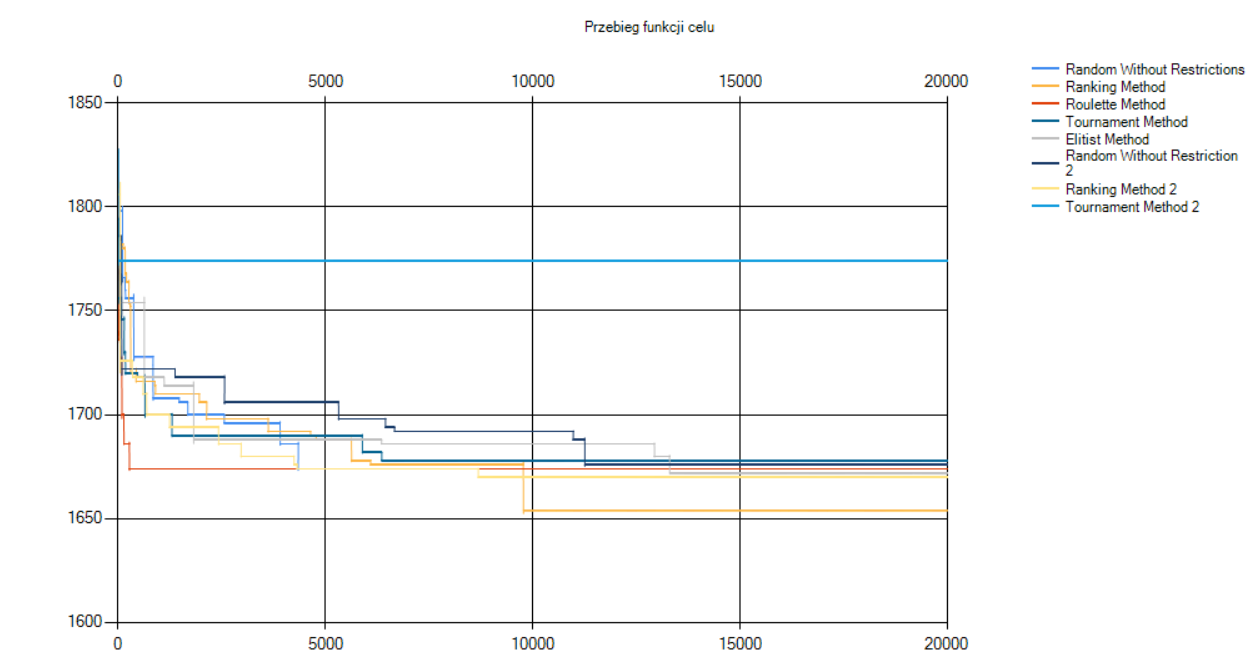
\includegraphics[scale=0.6]{../../../../Screeny/matody_1654_legend.png}
		\caption{Przebieg działania algorytmu dla~poszczególnych metod reprodukcji, 20 000 iteracji.}
		\label{ranking}			
\end{figure}

Na~podstawie wykresu \ref{instancja1} zauważalne staje się~zmniejszanie wartości funkcji celu w~kolejnych iteracjach algorytmu. W~przypadku metod takich jak~metoda ruletki czy~też metoda turniejowa, która~dopuszcza powtórzeń wśród osobników w~grupie rodzicielskiej, stabilizacja poziomu następuje w~początkowych iteracjach i~utrzymuje się~tak do~końca. Powodem tak~szybkiej zbieżności tych metod jest~brak różnorodności w~kolejnych grupach rodzicielskich. W~metodzie ruletki spowodowane jest~to~dużym prawdopodobieństwem wylosowania osobnika najlepszego, co prowadzi do~jego dominacji nad~innymi. Natomiast w~metodzie turniejowej turniej jest~w~większości przypadków wygrywany przez~tego samego osobnika, co przy dodatkowym założeniu, iż~w~jednej grupie rodzicielskiej mogą znajdować się~te~same osobniki prowadzi do~sytuacji w~której na~grupę rodzicielską składają się~3 te~same osobniki. Pomimo wrażenia, iż~rozwiązania osiągnęły stan stabilny już w~20 000 iteracji, należy sprawdzić, czy~nie nastąpi jeszcze spadek wartości funkcji celu, gdy liczba iteracji zostanie zwiększona. W~tym celu ponowione zostają badania metod dla~50 000 iteracji.\\

\subsubsection{50 000 iteracji}

 W~tabeli \ref{instancja2} zostały zestawione wartości błędu względnego funkcji celu w~kolejnych iteracjach dla~poszczególnych metod. W~metodach takich jak~metoda Losowa 2, Rankingowa 2 oraz~Turniejowa 2 nie~istnieje warunek co do~niepowtarzalności się~osobników w~obrębie jednej grupy rozrodczej. W~tym przypadku zwiększona została liczba iteracji działania algorytmu dla~każdej z~metod z~20 000 na~50 000. Kolorem zielonym zostały zaznaczone wyniki działania algorytmu osiągające wartość błędu względnego równą 0\%.

\begin{table}[h!]
\begin{center}
\caption{Wartości błędu względnego funkcji celu dla poszczególnych metod reprodukcji, 50 000 iteracji.}
\scalebox{0.6}{
\begin{tabular}{|c|c|c|c|c|c|c|c|c|}
\hline
\textbf{Iteracja}  &\textbf{Losowa}  & \textbf{Rankingowa} & \textbf{Ruletka} & \textbf{Turniejowa} & \textbf{Elitarna} & \textbf{Losowa 2} & \textbf{Rankingowa 2} & \textbf{Turniejowa 2}\\
\hline
 \textbf{1}&2,3 \%&0,6\%&4,47\%&0,24\%&1,21\%&2,66\%&1,93\%&4,6\% \\
\hline
 \textbf{2}&1,93\%&0,6\%&2,05\%&0,6\%&1,33\%&1,45\%&2,42\%&4,47\% \\
\hline
 \textbf{3}&0,24\%&1,81\%&1,93\%&1,33\%&1,93\%&1,21\%&1,21\%&6,29\%  \\
\hline
 \textbf{4}&3,99\%&0,24\%&1,81\%&1,21\%&1,45\%&2,42\%&0,48\%&7,99\%  \\
\hline
 \textbf{5}&2,3\%&0,6\%&1,21\%&0,96\%&2,05\%&4,47\%&1,45\%&8,35\%  \\
\hline
 \textbf{6}&1,69\%&0,48\%&4,47\%&2,3\%&1,45\%&2,54\%&1,21\%&9,2\%\\
\hline
 \textbf{7}&1,33\%&0,24\%&1,93\%&0,6\%&1,45\%&1,21\%&1,08\%&7,26\% \\
\hline
 \textbf{8}&2,42\%&0,84\%&1,81\%&0,96\%&0,72\%&1,39\%&2,05\%&6,77\%\\
\hline
 \textbf{9}&0,84\%&\color{green}\textbf{0\%}&0,6\%&0,72\%&1,08\%&2,05\%&2,42\%&8,83\%\\
\hline
 \textbf{10}&2,54\%&0,48\%&2,78\%&0,72\%&2,78\%&1,93\%&2,66\%&5,69\%\\
\hline
 \textbf{11}&2,54\%&0,24\%&1,69\%&1,33\%&1,45\%&3,14\%&3,14\%&3,87\%\\
\hline
 \textbf{12}&0,6 \%&0,48\%&2,05\%&0,48\%&0,6\%&2,66\%&0,96\%&10,53\%\\
\hline
 \textbf{13}&1,33\%&0,84\%&3,14\%&1,08\%&1,21\%&2,66\%&1,45\%&8,59\%\\
\hline
 \textbf{14}&0,84\%&0,24\%&2,3\%&1,45\%&1,21\%&4,47\%&1,21\%&5,69\%\\
\hline
 \textbf{15}&2,54\%&1,45\%&1,33\%&0,6\%&2,3\%&3,63\%&1,81\%&6,29\%\\
\hline
 \textbf{16}&1,08\%&0,6\%&2,66\%&0,96\%&1,81\%&1,45\%&1,08\%&10,53\%\\
\hline
 \textbf{17}&1,81\%&\color{green}\textbf{0\%}&1,33\%&0,72\%&1,21\%&3,99\%&0,48\%&9,2\%\\
\hline
 \textbf{18}&1,57\%&0,48\%&3,26\%&1,93\%&1,93\%&2,17\%&1,45\%&7,14\%\\
\hline
 \textbf{19}&1,08\%&0,48\%&1,57\%&0,84\%&2,3\%&3,99\%&0,96\%&6,53\%\\
\hline
 \textbf{20}&1,93\%&0,6\%&3,14\%&2,42\%&2,05\%&1,45\%&1,93\%&10,53\%\\
\hline
 \textbf{ŚREDNIA}&1,75\%&0,57\%&2,4\%&1,08\%&1,47\%&2,55\%&1,57\%&7,42\%\\
\hline
 \textbf{ODCHYLENIE STANDARDOWE}&0,85\%&0,42\%&0,93\%&0,57\%&0,51\%&1,06\%&0,7\%&1,99\%\\
\hline
\end{tabular}}
\label{instancja2}
\end{center}
\end{table}

W~przypadku 50 000 iteracji zauważalne jest~uzyskiwanie lepszych średnich wyników przez~metody takie jak: metoda rankingowa, metoda elitarna oraz~turniejowa dopuszczające istnienie powtórzeń w~grupie rodzicielskiej. Dzieje się~tak, ponieważ~metody te~nie kończą stabilizacji na~poziomie 20 000, a~spadek wartości funkcji celu następuje również w~dalszych iteracjach. Pozostałe metody utrzymały średnią na~tym samym bądź~też nieco wyższym poziomie w~stosunku to~próby testowej zakładającej 20 000 iteracji. Poniżej w~tabeli \ref{ranking2} zestawiony został ranking metod uporządkowany od~metody działającej najlepiej, na~pierwszym miejscu, do~metody działającej najmniej korzystnie, na~ostatnim.

\begin{table}[h!]
\begin{center}
\caption{Ranking metod reprodukcji na podstawie średniej wartości błędu względnego funkcji celu, 50 000 iteracji.}
\scalebox{0.8}{
\begin{tabular}{|c|c|c|c|}
\hline
\textbf{Miejsce}  &\textbf{Metoda}  & \textbf{Średni błąd względny funkcji celu} & \textbf{Liczba osiągnietych wartośći 0\%}\\
\hline
 \textbf{1}&Rankingowa&0,57\%& 2\\
\hline
 \textbf{2}&Turniejowa&1,08\%& 0\\
\hline
 \textbf{3}&Elitarna&1,47\%& 0\\
\hline
 \textbf{4}&Rankingowa 2&1,57\%& 0\\
\hline
 \textbf{5}&Losowa&1,75\%& 0\\
\hline
 \textbf{6}&Ruletki&2,4\%& 0\\
\hline
 \textbf{7}&Losowa 2&2,55\%& 0\\
\hline
 \textbf{8}&Turniejowa 2&7,42\%& 0\\
\hline
\end{tabular}}
\label{ranking2}
\end{center}
\end{table}

Na~podstawie tabeli \ref{ranking2} można wysunąć wniosek, iż~po raz kolejny najlepsze wyniki uzyskuje metoda rankingowa, a~zaraz po~niej powtórnie najkorzystniej zachowuje się~metoda turniejowa. Niemniej jednak przodowanie tych metod może mieć miejsce w~przypadku założonej instancji danych wejściowych, dlatego należy przeprowadzić testy przy użyciu innej macierzy odległości oraz~przepływu. Przebieg funkcji celu we wszystkich 50 000 iteracjach widoczny jest~na~wykresie \ref{ranking2picun}, na~którym to~zauważyć można również spadek dla~metody turniejowej, w~której istnieje zastrzeżenie co do~niepowtarzalności się~osobników w~grupie rozrodczej. Wyjątkowo niekorzystnym działaniem odznacza się~metoda Turniejowa 2, gdyż spadek następuje jedynie w~początkowych iteracjach i~na tym poziomie utrzymuje się~już do~końca.

\begin{figure}[h!]
		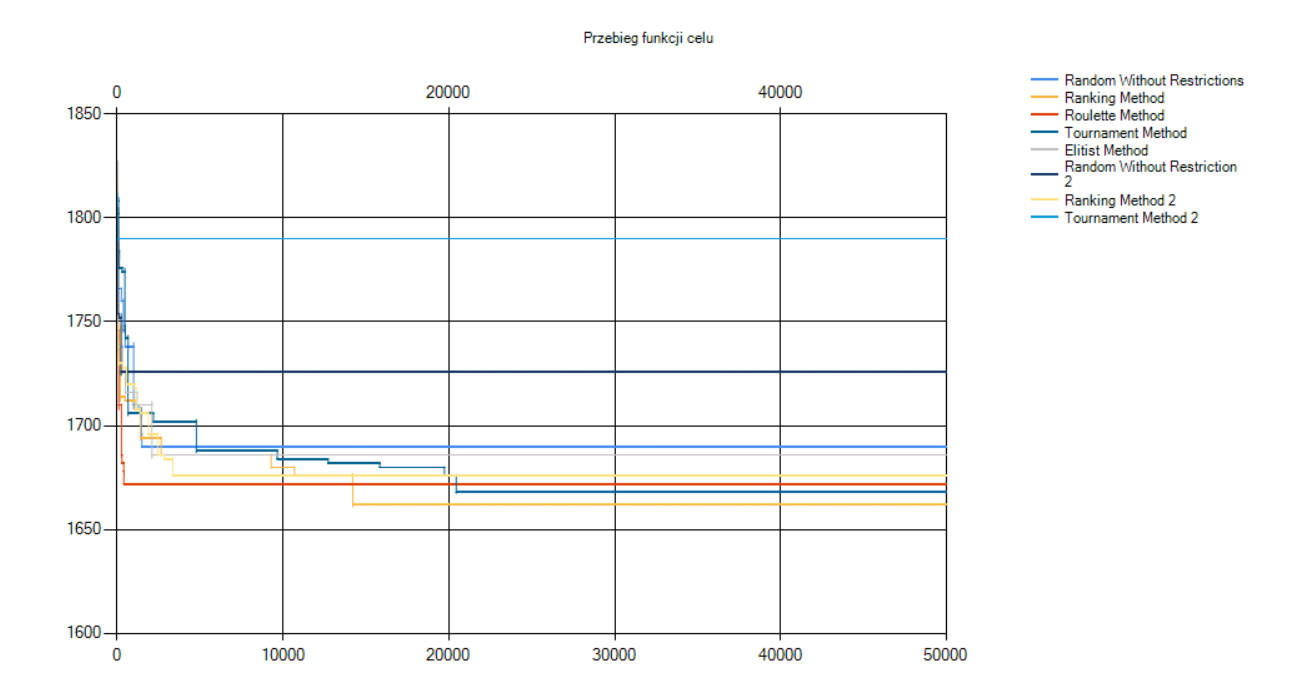
\includegraphics[scale=0.6]{../../../../Screeny/50_tys.png}
		\caption{Przebieg działania algorytmu dla~poszczególnych metod reprodukcji, 50 000 iteracji.}
		\label{ranking2picun}			
\end{figure}

Możliwe jest~zatem ustalenie optymalnej ilości iteracji na~liczbę 30 000, wówczas wartości funkcji celu w~poszczególnych metodach osiągną już stan stabilny, a~dodatkowe obliczenia dla~liczby równej aż 50 000 iteracji nie~będą musiały być~wykonywane.

\subsection{Metody mutacji}\label{mutacja}

Metody mutacji o~których mowa w~podrozdziale zostały szczegółowo opisane w~rozdziale 4. Testy metod mutacji w~obrębie jednej instancji danych zostały przeprowadzone przy uprzednim określeniu:
\begin{itemize}
\item
macierzy odległości,
\item
macierzy przepływu,
\item
metod reprodukcji,
\item
metoda krzyżowania,
\item
wielkość populacji,
\end{itemize}
\par
W~klasycznych metodach mutacji stosowany jest~wybór osobników do~grupy rozrodczej poprzez~metodę losową. Niemniej jednak ze~względu na~wyjątkowo dobre wyniki uzyskiwane przez~metodę rankingową w~testach przeprowadzanych w~rozdziale 6.1.1, postanowiono sprawdzić jej działanie w~połączeniu z~różnymi wariantami metod mutacji. Liczba iteracji algorytmu była równa, podobnie jak~w~powyższych testach, 20 000 iteracji. Następnie, w~celu zbadania czy~dalej niż granica 20 000 następuje spadek wartości funkcji celu, również dla~50 000 iteracji. Zgodnie z~podrozdziałem 4.2.4 metody mutacji zostaną dodatkowo przetestowane pod~kątem wpływu na~ich działanie parametru $\leftthreetimes$. Również dynamiczna zmiana parametru mutacji poddawana jest~testom.

%----------------------------------------------------------------------------------------------------------------------------------------------------------------------------------------------------

\subsubsection{Reprodukcja losowa}
W~rozdziale tym testy metod mutacji zostały przeprowadzone z~użyciem metody reprodukcji wykorzystywanej w~klasycznej wersji algorytmu ewolucji różnicowej. Metodą decydującą o~osobnikach wchodzących w~skład grupy rozrodczej jest~więc metoda losowa.\\
\par

\begin{itemize}
\item  \textbf{20 000 iteracji}\\

Wyniki zostały zaprezentowane w~formie tabeli zawierającej wartości błędu względnego funkcji celu. Testy przeprowadzono dla~20 powtórzeń algorytmu. W~wyniku tego działania możliwe było policzenie wartości średniej oraz~odchylenia standardowego z~kolejnych 20 prób.

\begin{table}[h!]
\begin{center}
\caption{Wartości błędu względnego funkcji celu dla poszczególnych metod mutacji, metoda losowa, 20 000 iteracji.}
\scalebox{0.55}{
\begin{tabular}{|c|c|c|c|c|c|c|c|c|}
\hline
\textbf{Iteracja}  &\textbf{DE/rand/1}  & \textbf{DE/rand/1+$\leftthreetimes$} & \textbf{DE/best/1} & \textbf{DE/best/1+$\leftthreetimes$} & \textbf{DE/rand/$n_{v}$} & \textbf{DE/rand/$n_{v}$+$\leftthreetimes$} & \textbf{ DE/current to best/$n_{v}+1$} & \textbf{ DE/current to best/$n_{v}+1$+$\leftthreetimes$}\\\hline
\textbf{1}&1,21\%&\color{green}\textbf{0}\%&3,39\%&1,94\%&0,85\%&0,48\%&0,73\%&0,61\% \\ \hline
\textbf{2}&0,97\%&0,61\%&4,84\%&0,85\%&1,21\%&1,33\%&0,61\%&0,73\% \\ \hline
\textbf{3}&2,91\%&0,61\%&2,66\%&1,21\%&1,33\%&0,85\%&0,12\%&0,12\% \\ \hline
\textbf{4}&2,18\%&1,33\%&1,33\%&1,45\%&1,82\%&0,61\%&0,61\%&1,09\% \\ \hline
\textbf{5}&2,06\%&2,42\%&2,42\%&3,51\%&1,57\%&1,69\%&1,09\%&0,24\% \\ \hline
\textbf{6}&1,57\%&1,94\%&2,54\%&1,82\%&0,85\%&0,24\%&0,85\%&0,24\% \\ \hline
\textbf{7}&3,15\%&1,69\%&3,75\%&0,85\%&2,54\%&1,09\%&1,09\%&0,48\% \\ \hline
\textbf{8}&1,57\%&1,21\%&3,39\%&0,85\%&1,45\%&1,69\%&1,21\%&0,48\% \\ \hline
\textbf{9}&1,82\%&4,84\%&5,08\%&1,82\%&0,97\%&0,48\%&0,61\%&0,61\% \\ \hline
\textbf{10}&1,33\%&0,61\%&4,24\%&1,69\%&1,33\%&2,18\%&0,48\%&\color{green}\textbf{0}\% \\ \hline
\textbf{11}&2,42\%&0,48\%&3,51\%&0,73\%&1,21\%&0,24\%&0,48\%&0,24\% \\ \hline
\textbf{12}&3,15\%&1,69\%&1,82\%&1,69\%&2,18\%&1,82\%&0,48\%&0,61\% \\ \hline
\textbf{13}&1,21\%&0,48\%&1,33\%&0,85\%&4,60\%&0,48\%&0,48\%&0,48\% \\ \hline
\textbf{14}&1,21\%&\color{green}\textbf{0}\%&3,03\%&1,21\%&1,33\%&0,85\%&0,97\%&0,24\% \\ \hline
\textbf{15}&1,21\%&0,48\%&1,45\%&0,97\%&1,45\%&0,48\%&1,21\%&0,61\% \\ \hline
\textbf{16}&0,61\%&1,33\%&2,30\%&1,21\%&0,48\%&2,91\%&0,85\%&0,12\% \\ \hline
\textbf{17}&1,94\%&0,48\%&4,24\%&3,39\%&0,61\%&\color{green}\textbf{0}\%&1,21&\color{green}\textbf{0}\% \\ \hline
\textbf{18}&3,15\%&0,48\%&2,42\%&2,06\%&2,18\%&2,42\%&0,48\%&0,85\% \\ \hline
\textbf{19}&4,24\%&1,94\%&6,17\%&1,45\%&0,85\%&3,75\%&0,61&\color{green}\textbf{0}\% \\ \hline
\textbf{20}&0,48\%&0,24\%&1,45\%&0,73\%&1,33\%&2,78\%&0,48\%&\color{green}\textbf{0}\% \\ \hline
\textbf{ŚREDNIA}&1,92\%&1,14\%&3,07\%&1,51\%&1,51\%&1,32\%&0,73\%&0,39\% \\ \hline
\textbf{ODCHYLENIE}&0,96\%&1,09\%&1,33\%&0,77\%&0,88\%&1,02\%&0,30\%&0,31\% \\ \hline
\end{tabular}}
\label{losowa20}
\end{center}
\end{table}

Sumaryczna liczba osiągnięcia przez~algorytm wartości błędu względnego równego 0\% jest~równa 7, z~czego 4 są~osiągane w~wyniku zastosowania w~algorytmie metody DE/current to~best/$n_{v}+1$.

\begin{table}[h!]
\begin{center}
\caption{Ranking metod mutacji na podstawie średniej wartości błędu względnego funkcji celu, metoda losowa, 20 000 iteracji.}
\scalebox{0.8}{
\begin{tabular}{|c|c|c|c|}
\hline
\textbf{Miejsce}  &\textbf{Metoda}  & \textbf{Średni błąd względny funkcji celu} & \textbf{Liczba osiągnietych wartośći 0\%}\\\hline
 \textbf{1}&DE/current to~best/$n_{v}+1$+$\leftthreetimes$&0,39\%& 4\\\hline
 \textbf{2}& DE/current to~best/$n_{v}+1$ &0,73\%& 0\\\hline
 \textbf{3}&DE/rand/$n_{v}$+$\leftthreetimes$&1,14\%& 1\\\hline
 \textbf{4}&DE/rand/1+$\leftthreetimes$&1,32\%& 2\\\hline
 \textbf{5}&DE/rand/$n_{v}$&1,51\%&0\\\hline
 \textbf{6}&DE/best/1+$\leftthreetimes$1&1,51\%& 0\\\hline
 \textbf{7}&DE/rand/1&1,92\%& 0\\\hline
 \textbf{8}&DE/best/1&3,07\%& 0\\\hline
\end{tabular}}
\label{ranking5}
\end{center}
\end{table}

Na~podstawie tabeli \ref{ranking5} widoczny staje się~fakt, iż~najmniejszą średnią wartością błędu względnego, o~wartości 0,39\%, charakteryzuje się~metoda DE/current to~best/$n_{v}+1$+$\leftthreetimes$. W~zestawieniu z~pozostałymi metodami mutacji przyjmuje ona około dwukrotnie lepsze rezultaty, jako, że~pozostałe metody uzyskują wartości błędu względnego wahające się~w~zakresie 0,73\% - 3,07\%. Wartość odchylenia standardowego dla~tej metody wynosi 0,31\% co w~porównaniu z~pozostałymi testowanymi metodami mutacji jest~wartością stosunkowo niewielką. Metoda DE/current to~best/$n_{v}+1$+$\leftthreetimes$ uzyskuje korzystniejsze rezultaty w~porównaniu do~jej odpowiednika bez modyfikatora DE/current to~best/$n_{v}+1$. W~przypadku pozostałych metod, DE/rand/$n_{v}$, DE/rand/1 oraz~DE/best/1, modyfikacja współczynnikiem $\leftthreetimes$ również pozwala na~uzyskiwanie przez~te metody bardziej zadowalających efektów.\\


\item  \textbf{50 000 iteracji}\\

Poniższe testy w~stosunku do~poprzednich zestawionych w~tabelach \ref{losowa20} oraz~\ref{ranking5} różnią się~od~siebie liczbą iteracji algorytmu, zwiększoną z~20 000 do~50 000. Działanie to~wprowadzone jest~w~celu zbadania czy~nie następuje spadek wartości funkcji celu w~iteracjach dalszych niż 20 000. Dodatkowym atutem jest~możliwość konfrontacji wyników, a~więc sprawdzenia, czy~uzyskane w~poprzednich testach wartości utrzymują się~na~tym samy bądź~też lepszym poziomie.

\begin{table}[h!]
\begin{center}
\caption{Wartości błędu względnego funkcji celu dla poszczególnych metod mutacji, metoda losowa, 50 000 iteracji.}
\scalebox{0.55}{
\begin{tabular}{|c|c|c|c|c|c|c|c|c|}
\hline
\textbf{Iteracja}  &\textbf{DE/rand/1}  & \textbf{DE/rand/1+$\leftthreetimes$} & \textbf{DE/best/1} & \textbf{DE/best/1+$\leftthreetimes$} & \textbf{DE/rand/$n_{v}$} & \textbf{DE/rand/$n_{v}$+$\leftthreetimes$} & \textbf{ DE/current to best/$n_{v}+1$} & \textbf{ DE/current to best/$n_{v}+1$+$\leftthreetimes$}\\\hline
\textbf{1}&1,09\%&0,85\%&2,06\%&2,91\%&0,85\%&1,57\%&0,12\%&\color{green}\textbf{0}\% \\ \hline
\textbf{2}&1,82\%&0,48\%&2,91\%&2,06\%&0,73\%&1,09\%&0,48\%&\color{green}\textbf{0}\% \\ \hline
\textbf{3}&1,57\%&1,45\%&1,82\%&2,54\%&1,57\%&0,48\%&0,12\%&0,48\% \\ \hline
\textbf{4}&0,97\%&0,85\%&2,54\%&2,54\%&1,45\%&0,61\%&0,24\%&\color{green}\textbf{0}\% \\ \hline
\textbf{5}&2,91\%&0,73\%&2,18\%&0,73\%&0,85\%&0,73\%&\color{green}\textbf{0}\%&0,48\% \\ \hline
\textbf{6}&1,09\%&1,82\%&2,54\%&0,48\%&1,45\%&1,69\%&0,61\%&0,97\% \\ \hline
\textbf{7}&0,73\%&2,06\%&3,27\%&1,94\%&1,21\%&2,42\%&0,48\%&\color{green}\textbf{0}\% \\ \hline
\textbf{8}&2,66\%&8,23\%&2,06\%&2,30\%&2,06\%&0,61\%&0,48\%&0,12\% \\ \hline
\textbf{9}&1,57\%&1,82\%&1,94\%&1,33\%&0,61\%&2,54\%&0,61\%&\color{green}\textbf{0}\% \\ \hline
\textbf{10}&1,94\%&2,42\%&1,21\%&1,09\%&1,45\%&0,97\%&0,12\%&\color{green}\textbf{0}\% \\ \hline
\textbf{11}&2,66\%&1,82\%&2,06\%&2,30\%&0,85\%&0,24\%&0,61\%&0,24\% \\ \hline
\textbf{12}&\color{green}\textbf{0}\%&3,51\%&4,36\%&2,54\%&2,30\%&\color{green}\textbf{0}\%&0,12\%&0,12\% \\ \hline
\textbf{13}&0,48\%&0,12\%&1,82\%&2,18\%&1,45\%&\color{green}\textbf{0}\%&0,48\%&\color{green}\textbf{0}\% \\ \hline
\textbf{14}&0,97\%&0,12\%&1,45\%&2,42\%&1,94\%&1,94\%&0,24\%&0,12\% \\ \hline
\textbf{15}&0,85\%&0,61\%&2,78\%&2,91\%&1,33\%&0,61\%&0,24\%&0,73\% \\ \hline
\textbf{16}&1,09\%&0,48\%&5,08\%&0,85\%&0,61\%&3,27\%&0,48\%&0,24\% \\ \hline
\textbf{17}&2,06\%&\color{green}\textbf{0}\%&2,42\%&1,57\%&0,85\%&1,21\%&0,48\%&0,12\% \\ \hline
\textbf{18}&0,48\%&\color{green}\textbf{0}\%&2,30\%&2,66\%&0,61\%&1,57\%&0,48\%&0,48\% \\ \hline
\textbf{19}&5,57\%&\color{green}\textbf{0}\%&2,78\%&2,30\%&6,90\%&\color{green}\textbf{0}\%&0,48\%&0,24\% \\ \hline
\textbf{20}&1,94\%&0,12\%&3,27\%&1,69\%&0,61\%&1,09\%&0,24\%&\color{green}\textbf{0}\% \\ \hline
\textbf{ŚREDNIA}&1,62\%&1,37\%&2,54\%&1,97\%&1,48\%&1,13\%&0,36\%&0,22\% \\ \hline
\textbf{ODCHYLENIE}&1,19\%&1,83\%&0,90\%&0,72\%&1,34\%&0,88\%&0,19\%&0,27\% \\ \hline
\end{tabular}}
\label{losowa50}
\end{center}
\end{table}

Liczba próbek, w~których algorytm uzyskiwał wartość błędu względnego równą 0\% wzrosła o~9 w~stosunku do~wersji algorytmu z~liczbą iteracji równą 20 000. Świadczy to~o~zmniejszaniu się~wartość funkcji celu w~iteracjach dalszych niż 20 000. W~przypadku większości z~metod następuje spadek średniej wartości błędu bezwzględnego funkcji celu. Niemniej jednak w~przypadku metod takich jak~DE/rand/1+$\leftthreetimes$ oraz~DE/best/1+$\leftthreetimes$ następuje wzrost tej wartości. Zjawisko to~spowodowane jest~zadziałaniem czynnika losowego. 

\begin{table}[h!]
\begin{center}
\caption{Ranking metod mutacji na podstawie średniej wartości błędu względnego funkcji celu, metoda losowa, 50 000 iteracji.}
\scalebox{0.8}{
\begin{tabular}{|c|c|c|c|}
\hline
\textbf{Miejsce}  &\textbf{Metoda}  & \textbf{Średni błąd względny funkcji celu} & \textbf{Liczba osiągnietych wartośći 0\%}\\\hline
 \textbf{1}&DE/current to~best/$n_{v}+1$ +$\leftthreetimes$&0,22\%& 8\\\hline
 \textbf{2}& DE/current to~best/$n_{v}+1$&0,36\%& 1\\\hline
 \textbf{3}&DE/rand/$n_{v}$+$\leftthreetimes$&1,13\%& 3\\\hline
 \textbf{4}&DE/rand/1+$\leftthreetimes$&1,37\%& 3\\\hline
 \textbf{5}&DE/rand/$n_{v}$&1,48\%&0\\\hline
 \textbf{6}&DE/rand/1&1,62\%&1\\\hline
 \textbf{7}&DE/best/1+$\leftthreetimes$&1,97\%& 0\\\hline
 \textbf{8}&DE/best/1&2,54\%& 0\\\hline
\end{tabular}}
\label{ranking3}
\end{center}
\end{table}

Na~podstawie tabeli będącej zestawieniem wszystkich testowanych metod mutacji, tabela \ref{ranking3}, potwierdza się~zauważona w~poprzednich testach zależność, iż~najlepiej działającą metodą jest~metoda DE/current to~best/$n_{v}+1$+$\leftthreetimes$. Średni błąd względny jest~równy 0,22\%, co jest~wartością około dwukrotnie mniejszą od~wyników uzyskiwanych przez~inne metody mutacji.

\end{itemize}

%----------------------------------------------------------------------------------------------------------------------------------------------------------------------------------------------------


\subsubsection{Reprodukcja rankingowa}
W~poniżej przeprowadzonej analizie za~metodę reprodukcji przyjmuje się~metodę rankingową. Testy zostaną przeprowadzone zarówno dla~20 000, jak~i~dla 50 000 iteracji.\\
\par
\begin{itemize}
\item  \textbf{20 000 iteracji}\\
\par
Analiza wyników przeprowadzona zostanie w~oparciu o~sprowadzenie uzyskanych wartości funkcji celu do~postaci ich błędu względnego. Liczba iteracji algorytmu jest~równa 20 000.

\begin{table}[h!]
\begin{center}
\caption{Wartości błędu względnego funkcji celu dla poszczególnych metod mutacji, metoda rankingowa, 20 000 iteracji.}
\scalebox{0.55}{
\begin{tabular}{|c|c|c|c|c|c|c|c|c|}
\hline
\textbf{Iteracja}  &\textbf{DE/rand/1}  & \textbf{DE/rand/1+$\leftthreetimes$} & \textbf{DE/best/1} & \textbf{DE/best/1+$\leftthreetimes$} & \textbf{DE/rand/$n_{v}$} & \textbf{DE/rand/$n_{v}$+$\leftthreetimes$} & \textbf{ DE/current to best/$n_{v}+1$} & \textbf{ DE/current to best/$n_{v}+1$+$\leftthreetimes$}\\
\hline
\textbf{1}&0,85\%&0,73\%&1,21\%&1,33\%&0,61\%&0,24\%&0,24\%&0,48\% \\ \hline
\textbf{2}&1,09\%&0,24\%&1,82\%&1,09\%&0,73\%&0,48\%&0,24\%&0,61\% \\ \hline
\textbf{3}&0,48\%&0,24\%&2,06\%&2,54\%&0,73\%&0,48\%&0,85\%&0,24\% \\ \hline
\textbf{4}&0,48\%&0,24\%&1,33\%&0,48\%&0,24\%&0,48\%&0,48\%&0,48\% \\ \hline
\textbf{5}&0,73\%&0,73\%&0,48\%&0,48\%&0,61\%&0,24\%&0,24\%&0,48\% \\ \hline
\textbf{6}&1,09\%&0,85\%&2,78\%&1,21\%&0,48\%&0,61\%&0,24\%&0,48\% \\ \hline
\textbf{7}&0,85\%&0,48\%&1,33\%&1,21\%&0,85\%&0,48\%&0,24\%&0,12\% \\ \hline
\textbf{8}&1,21\%&0,48\%&0,48\%&1,57\%&1,82\%&0,24\%&0,24\%&0,48\% \\ \hline
\textbf{9}&0,24\%&0,61\%&1,21\%&1,57\%&0,85\%&1,09\%&0,48\%&0,85\% \\ \hline
\textbf{10}&1,33\%&0,73\%&1,33\%&1,21\%&1,09\%&0,48\%&0,61\%&\color{green}\textbf{0}\% \\ \hline
\textbf{11}&0,85\%&\color{green}\textbf{0}\%&0,85\%&1,33\%&0,12\%&0,12\%&1,09\%&\color{green}\textbf{0}\% \\ \hline
\textbf{12}&0,24\%&0,48\%&1,69\%&1,57\%&0,97\%&0,48\%&\color{green}\textbf{0}\%&0,48\% \\ \hline
\textbf{13}&0,73\%&0,85\%&0,61\%&1,57\%&0,61\%&0,48\%&0,24\%&1,09\% \\ \hline
\textbf{14}&0,48\%&0,12\%&0,97\%&1,33\%&0,48\%&0,24\%&1,21\%&0,85\% \\ \hline
\textbf{15}&\color{green}\textbf{0}\%&0,24\%&0,48\%&0,61\%&1,21\%&0,24\%&\color{green}\textbf{0}\%&\color{green}\textbf{0}\% \\ \hline
\textbf{16}&0,48\%&0,61\%&2,30\%&1,69\%&0,61\%&0,73\%&0,48\%&\color{green}\textbf{0}\% \\ \hline
\textbf{17}&0,61\%&0,12\%&2,54\%&2,18\%&0,48\%&0,61\%&0,24\%&0,61\% \\ \hline
\textbf{18}&1,82\%&0,61\%&2,18\%&1,33\%&0,48\%&0,48\%&0,48\%&0,61\% \\ \hline
\textbf{19}&1,09\%&0,24\%&1,21\%&1,21\%&1,57\%&0,48\%&0,61\%&0,48\% \\ \hline
\textbf{20}&0,73\%&0,61\%&2,66\%&0,85\%&0,48\%&0,48\%&0,73\%&0,48\% \\ \hline
\textbf{ŚREDNIA}&0,77\%&0,46\%&1,48\%&1,32\%&0,75\%&0,46\%&0,45\%&0,44\% \\ \hline
\textbf{ODCHYLENIE}&0,41\%&0,25\%&0,73\%&0,49\%&0,41\%&0,21\%&0,32\%&0,30\% \\ \hline
\end{tabular}}
\label{rankingowa20}
\end{center}
\end{table}
\par
Analizując tabele \ref{rankingowa20} widoczny staje się~fakt, iż~najlepsze wyniki uzyskiwane są~dla strategii DE/current to~best/$n_{v}+1$+$\leftthreetimes$, jako że~aż 4 razy algorytm z~udziałem tej metody mutacji osiągał błąd względy równy 0\%. W~pozostałych iteracjach wartości błędu względnego w~przeważającej części również były niewielkie, wartości te~wahają się~w~zakresie (0,1,48\%). Współczynnik odchylenia standardowego dla~wspomnianej powyżej metody jest~równy 0,3 \%, co świadczy o~bliskim skupieniu wartości w~poszczególnych iteracjach wokół średniej. Jest~to~również jedna z~mniejszych wartości odchylenia standardowego, biorąc pod~uwagę wartości uzyskiwane przez~inne metody mutacji.\\
Strategia DE/current to~best/$n_{v}+1$ nie~uwzględniająca zależności opisanych w~podrozdziale 4.2.4, a~więc bez wprowadzenia dodatkowego współczynnika $\leftthreetimes$, także przynosi satysfakcjonujące wyniki. Średni błąd względny wynosi 0,45\%, a~algorytm 2 razy doprowadza funkcję celu do~wartości uznawanej przez~\cite{qaplib} za~najmniejszą znaną wartość. W~tabeli \ref{ranking3} został przedstawiony ranking metod mutacji ułożony w~zależności od~uzyskanej przez~metody te~średniej wartości błędu względnego.

\begin{table}[h!]
\begin{center}
\caption{Ranking metod mutacji na podstawie średniej wartości błędu względnego funkcji celu, metoda rankingowa, 20 000 iteracji.}
\scalebox{0.8}{
\begin{tabular}{|c|c|c|c|}
\hline
\textbf{Miejsce}  &\textbf{Metoda}  & \textbf{Średni błąd względny funkcji celu} & \textbf{Liczba osiągnietych wartośći 0\%}\\\hline
 \textbf{1}&DE/current to~best/$n_{v}+1$+$\leftthreetimes$&0,44\%& 4\\\hline
 \textbf{2}& DE/current to~best/$n_{v}+1$&0,45\%& 2\\\hline
 \textbf{3}&DE/rand/$n_{v}$+$\leftthreetimes$&0,46\%& 0\\\hline
 \textbf{4}&DE/rand/1+$\leftthreetimes$&0,46\%& 1\\\hline
 \textbf{5}&DE/rand/$n_{v}$&0,75\%&0\\\hline
 \textbf{6}&DE/rand/1&0,77\%& 1\\\hline
 \textbf{7}&DE/best/1+$\leftthreetimes$&1,32\%& 0\\\hline
 \textbf{8}&DE/best/1&1,48\%& 0\\\hline
\end{tabular}}
\label{ranking6}
\end{center}
\end{table}

Na~podstawie tabeli \ref{ranking3} można wysnuć wniosek, iż~metody takie jak~ DE/current to~best/$n_{v}+1$+$\leftthreetimes$,  DE/rand/$n_{v}$+$\leftthreetimes$,  DE/rand/1+$\leftthreetimes$ oraz~DE/best/1+$\leftthreetimes$, a~wiec metody, które~zostały zmodyfikowane współczynnikiem $\leftthreetimes$ uzyskują korzystniejsze wyniki w~porównaniu do~ich odpowiedników bez modyfikatora. Widoczna staje się~zatem skuteczność działania czynnika skalującego $\leftthreetimes$.\\

\item  \textbf{50 000 iteracji }

Poniższe testy zostały przeprowadzone w~celu zbadania czy~uzyskane wyniki utrzymają się~na~poziomie, który~osiągają na~etapie 20 000 iteracji, czy~też następuje poprawa w~sytuacji zwiększenia liczby iteracji. Wyniki testów zestawiono w~tabeli \ref{rankingowa50}.\\

\begin{table}[h!]
\begin{center}
\caption{Wartości błędu względnego funkcji celu dla poszczególnych metod mutacji, metoda rankingowa, 50 000 iteracji.}
\scalebox{0.55}{
\begin{tabular}{|c|c|c|c|c|c|c|c|c|}
\hline
\textbf{Iteracja}  &\textbf{DE/rand/1}  & \textbf{DE/rand/1+$\leftthreetimes$} & \textbf{DE/best/1} & \textbf{DE/best/1+$\leftthreetimes$} & \textbf{DE/rand/$n_{v}$} & \textbf{DE/rand/$n_{v}$+$\leftthreetimes$} & \textbf{ DE/current to best/$n_{v}+1$} & \textbf{ DE/current to best/$n_{v}+1$+$\leftthreetimes$}\\
\hline
\textbf{1}&1,33\%&0,85\%&1,33\%&1,33\%&0,24\%&0,48\%&0,12\%&0,48\% \\ \hline
\textbf{2}&0,85\%&\color{green}\textbf{0}\%&1,21\%&0,97\%&0,61\%&0,12\%&0,61\%&0,48\% \\ \hline
\textbf{3}&0,73\%&1,57\%&1,57\%&0,61\%&0,48\%&0,24\%&0,24\%&0,12\% \\ \hline
\textbf{4}&0,97\%&0,48\%&1,33\%&1,45\%&\color{green}\textbf{0}\%&0,48\%&0,97\%&0,12\% \\ \hline
\textbf{5}&0,48\%&0,24\%&0,61\%&1,45\%&0,61\%&0,24\%&0,24\%&\color{green}\textbf{0}\% \\ \hline
\textbf{6}&0,73\%&0,48\%&1,09\%&2,54\%&0,12\%&\color{green}\textbf{0}\%&\color{green}\textbf{0}\%&0,48\% \\ \hline
\textbf{7}&0,24\%&0,24\%&2,78\%&0,85\%&0,48\%&0,48\%&0,85\%&0,12\% \\ \hline
\textbf{8}&0,48\%&0,48\%&1,09\%&2,18\%&0,48\%&0,24\%&\color{green}\textbf{0}\%&0,24\% \\ \hline
\textbf{9}&0,24\%&0,48\%&2,06\%&0,61\%&0,48\%&0,48\%&0,24\%&0,48\% \\ \hline
\textbf{10}&0,85\%&0,48\%&1,57\%&1,33\%&0,48\%&0,48\%&0,24\%&1,09\% \\ \hline
\textbf{11}&2,18\%&0,48\%&1,94\%&2,18\%&0,61\%&0,24\%&0,24\%&0,12\% \\ \hline
\textbf{12}&\color{green}\textbf{0}\%&0,61\%&2,78\%&1,69\%&0,48\%&\color{green}\textbf{0}\%&0,24\%&0,24\% \\ \hline
\textbf{13}&0,73\%&0,73\%&1,21\%&1,45\%&0,48\%&0,48\%&0,24\%&0,48\% \\ \hline
\textbf{14}&\color{green}\textbf{0}\%&0,24\%&3,03\%&1,09\%&0,48\%&0,73\%&0,24\%&0,24\% \\ \hline
\textbf{15}&0,48\%&\color{green}\textbf{0}\%&1,33\%&1,09\%&0,85\%&\color{green}\textbf{0}\%&0,12\%&0,24\% \\ \hline
\textbf{16}&0,48\%&0,61\%&1,09\%&1,45\%&\color{green}\textbf{0}\%&0,24\%&0,48\%&0,24\% \\ \hline
\textbf{17}&0,73\%&0,24\%&1,94\%&1,69\%&0,61\%&0,48\%&0,48\%&\color{green}\textbf{0}\% \\ \hline
\textbf{18}&0,61\%&1,09\%&1,82\%&1,57\%&0,48\%&0,61\%&0,61\%&0,24\% \\ \hline
\textbf{19}&0,73\%&0,48\%&1,09\%&1,82\%&0,12\%&0,12\%&\color{green}\textbf{0}\%&0,24\% \\ \hline
\textbf{20}&0,61\%&0,73\%&2,66\%&1,69\%&\color{green}\textbf{0}\%&\color{green}\textbf{0}\%&0,48\%&0,24\% \\ \hline
\textbf{ŚREDNIA}&0,67\%&0,53\%&1,68\%&1,45\%&0,41\%&0,31\%&0,33\%&0,30\% \\ \hline
\textbf{ODCHYLENIE}&0,46\%&0,35\%&0,67\%&0,49\%&0,23\%&0,22\%&0,26\%&0,24\% \\ \hline
\end{tabular}}
\label{rankingowa50}
\end{center}
\end{table}
\par

Wartości błędu względnego dla~danych metod uległy poprawie w~stosunku do~ograniczenia liczby iteracji do~20 000. Wynika to~z~faktu, iż~po przekroczeniu tej granicy, w~grupach rodzicielskich nadal występują osobniki o~różnym od~siebie genotypie. Zjawisko to~prowadzi do~polepszania się~wartości funkcji dopasowania. Analizując przebiegi \ref{rankingowa50pic} można zauważyć, iż~stan stabilny utrzymuje się~dopiero na~poziomie 30 000 iteracji, co widoczne jest~na~poniższym wykresie.

\begin{figure}[h!]
		\includegraphics[scale=0.6]{../../../../Screeny/50000_2metody_1652.png}
		\caption{Przebieg działania algorytmu dla~poszczególnych metod mutacji.}
		\label{rankingowa50pic}			
\end{figure}

Poniżej zamieszczono zestawienie funkcji uporządkowanych w~kolejności zależnej od~uzyskanej przez~metody te~wartości błedu względnego funkcji celu.

\begin{table}[h!]
\begin{center}
\caption{Ranking metod mutacji na podstawie średniej wartości błędu względnego funkcji celu, metoda rankingowa, 50 000 iteracji.}
\scalebox{0.8}{
\begin{tabular}{|c|c|c|c|}
\hline
\textbf{Miejsce} &\textbf{Metoda}  & \textbf{Średni błąd względny funkcji celu} & \textbf{Liczba osiągnietych wartośći 0\%}\\\hline
 \textbf{1}& DE/current to~best/$n_{v}+1$+$\leftthreetimes$&0,3\%& 2\\\hline
 \textbf{2}& DE/rand/$n_{v}$+$\leftthreetimes$&0,31\%& 4\\\hline
 \textbf{3}& DE/current to~best/$n_{v}+1$&0,33\%& 3\\\hline
 \textbf{4}& DE/rand/$n_{v}$&0,41\%& 3\\\hline
 \textbf{5}& DE/rand/1+$\leftthreetimes$&0,53\%&2\\\hline
 \textbf{6}& DE/rand/1&0,67\%&2\\\hline
 \textbf{7}& DE/best/1+$\leftthreetimes$&1,45\%& 0\\\hline
 \textbf{8}& DE/best/1&1,68\%& 0\\\hline
\end{tabular}}
\label{ranking4}
\end{center}
\end{table}

Ranking dla~50 000 iteracji zmienił się~w~stosunku do~rankingu 20 000 iteracji nie~tylko w~kontekście mniejszych wartości błędu względnego dla~niektórych z~funkcji, ale~również w~kontekście pozycji zajmowanych przez~metody w~rankingu. Nadal najlepsze wyniki uzyskiwane są~dla metody DE/current to~best/$n_{v}+1$+$\leftthreetimes$. Błąd względny tej metody zmniejszył się~o~0,14 \% w~stosunku do~jej działania z~użyciem algorytmu, w~którym liczba iteracji była ustalona na~wartość 20 000. Podobne wyniki uzyskują również metody DE/rand/$n_{v}$+$\leftthreetimes$ orazDE/current to~best/$n_{v}+1$, zajmując tym samym odpowiednio drugie oraz~trzecie miejsce w~rankingu. Niezależnie od~zastosowanej metody reprodukcji metody DE/best/1+$\leftthreetimes$ oraz~DE/best/1 odznaczają się~wyjątkowo niekorzystnymi wynikami w~porównaniu z~pozostałymi metodami mutacji. Uzyskiwane przez~metody te~wyniki są~około dwukrotnie gorsze.\\

\end{itemize}

%----------------------------------------------------------------------------------------------------------------------------------------------------------------------------------

\subsection{Metody krzyżowania}\label{crossover}

Metody krzyżowania, o~których mowa w~podrozdziale zostały szczegółowo opisane w~rozdziale 5. Metody krzyżowania zostały przetestowane w~każdym z~podrozdziałów przy założeniu stałych takich jak:
\begin{itemize}
\item macierz odległości,
\item macierz przepływu,
\item metoda reprodukcji,
\item metoda mutacji,
\item wielkość populacji
\end{itemize}
\par
Testy zostały podzielone na~trzy główne bloki. Pierwszy z~nich zakłada uznanie za~metodę reprodukcji klasyczną metodę losową, natomiast za~metodę mutacji strategie DE/rand/1. W~kolejnych dwóch blokach testowych zostały uwzględnione wyniki otrzymane w~wyżej przeprowadzonych testach. Poprzez~zestawienie z~metodami krzyżowania, możliwe było dokonanie sprawdzenia jaka kombinacja metod z~poszczególnych sekcji algorytmu pozwoli na~osiągnięcie najbardziej satysfakcjonujących wyników. Dane początkowe, dla~których przeprowadzono testy, znajdują się~w~rozdziale 7.1.1. Dodatkowo zgodnie z~informacjami zawartymi w~podrozdziale \ref{dostrajaniecr} zostanie przebadany wpływ współczynnika krzyżowania $C_{r}$ na~działanie poszczególnych metod.\\

\subsubsection{Reprodukcja losowa, mutacja DE/rand/1}

W~przypadku metod krzyżowania testy zostaną przeprowadzone, zgodnie z~przyjętym sposobem prowadzenia testów dla~metod selekcji oraz~metod mutacji, dla~20 000 iteracji, a~następnie dla~50 000 iteracji. Metoda losowa oraz~strategia DE/rand/1 stanowi klasyczną wersję algorytmu ewolucji różnicowej, testy z~użyciem tych metod są~przeprowadzane w~celu konfrontacji wyników działania wersji klasycznej z~wynikami działania metod zmutowanych.\\

\begin{itemize}
\item  \textbf{20 000 iteracji}

Testy dla~każdej z~metod krzyżowania zostały przeprowadzone 20 razy, a~następnie na~podstawie uzyskanych wartości została obliczona wartość podstawowych miar statystycznych takich jak~średnia i~odchylenie standardowe. Na~podstawie tych wartości oceniona została skuteczność działania poszczególnych metod. Wyniki uzyskiwane w~kolejnych iteracjach przez~poszczególne metody zostały zestawione w~poniższej tabeli. Zapisane są~one w~formie wartości błędu względnego z~uzyskanego wyniku.\\
\par
\begin{table}[h!]
\begin{center}
\caption{Wartości błędu względnego funkcji celu dla poszczególnych metod krzyżowania, reprodukcja losowa,  mutacja DE/rand/1, 20 000 iteracji.}
\scalebox{0.55}{
\begin{tabular}{|c|c|c|c|c|}
\hline
\textbf{Iteracja}  &\textbf{Dwumianowe}  & \textbf{OX} & \textbf{CX} & \textbf{PMX}\\
\hline
\textbf{1}&2,30\%&1,09\%&4,36\%&10,53\% \\ \hline
\textbf{2}&1,94\%&1,33\%&2,91\%&4,96\% \\ \hline
\textbf{3}&0,24\%&0,61\%&2,78\%&11,86\% \\ \hline
\textbf{4}&1,33\%&1,21\%&2,18\%&11,50\% \\ \hline
\textbf{5}&1,82\%&0,48\%&2,30\%&7,02\% \\ \hline
\textbf{6}&3,15\%&1,09\%&2,42\%&9,32\% \\ \hline
\textbf{7}&1,21\%&1,45\%&2,66\%&8,11\% \\ \hline
\textbf{8}&3,27\%&0,48\%&3,39\%&8,47\% \\ \hline
\textbf{9}&0,48\%&1,45\%&1,82\%&11,14\% \\ \hline
\textbf{10}&2,91\%&0,12\%&2,91\%&8,72\% \\ \hline
\textbf{11}&0,73\%&0,85\%&2,18\%&9,44\% \\ \hline
\textbf{12}&0,61\%&0,48\%&4,84\%&10,05\% \\ \hline
\textbf{13}&0,97\%&0,24\%&5,21\%&8,84\% \\ \hline
\textbf{14}&1,57\%&1,09\%&3,27\%&9,93\% \\ \hline
\textbf{15}&0,85\%&1,57\%&3,51\%&9,56\% \\ \hline
\textbf{16}&1,21\%&2,18\%&2,54\%&5,21\% \\ \hline
\textbf{17}&1,57\%&0,97\%&1,21\%&9,69\% \\ \hline
\textbf{18}&0,24\%&1,09\%&2,91\%&7,14\% \\ \hline
\textbf{19}&0,97\%&0,73\%&2,42\%&8,96\% \\ \hline
\textbf{20}&0,97\%&0,85\%&4,36\%&8,47\% \\ \hline
\textbf{ŚREDNIA}&1,42\%&0,97\%&3,01\%&8,95\% \\ \hline
\textbf{ODCHYLENIE}&0,89\%&0,49\%&1,00\%&1,79\% \\ \hline
\end{tabular}}
\label{klasyczna20}
\end{center}
\end{table}

Zauważalny staje się~fakt, iż~w~przypadku wykonywania się~programu przez~20 000 iteracji, nie~udało się~żadnej ze~strategii osiągnąć wartości błędu względnego równej 0\%. Spośród dostępnych metod najlepsze rezultaty uzyskuje metoda OX, jako że~wartość błędu jest~równa 0,97 \%. Wynik działania strategii krzyżowania dwumianowego znajduje się~w~niewielkim otoczeniu od~wyniku uzyskanego przez~krzyżowanie dwumianowe. Z~koleii metody CX oraz~PMX odznaczają się~wyjątkowo dużą wartością błędu względnego, rzędu (3,9 \%). Uporządkowany układ od~najmniejszej do~największej wartości średniego błędu względnego został przedstawiony poniżej.

\begin{table}[h!]
\begin{center}
\caption{Ranking metod krzyżowania na podstawie średniej wartości błędu względnego funkcji celu, reprodukcja losowa,  mutacja DE/rand/1, 20 000 iteracji.}
\scalebox{0.8}{
\begin{tabular}{|c|c|c|c|}
\hline
\textbf{Miejsce}  &\textbf{Metoda}  & \textbf{Średni błąd względny funkcji celu} & \textbf{Liczba osiągnietych wartośći 0\%}\\\hline
 \textbf{1}&OX&0,97\%& 0\\\hline
 \textbf{2}&Dwumianowe&1,42\%& 0\\\hline
 \textbf{3}&CX&3,01\%& 0\\\hline
 \textbf{4}&PMX&8,95\%&0\\\hline
\end{tabular}}
\label{rankingcross1}
\end{center}
\end{table}

\item \textbf{50 000 iteracji}
Niezadowalające efekty działania algorytmu uwzględniającego w~swoim działaniu metody krzyżowania CX czy~też PMX mogą poniekąd wynikać z~niewystarczająco dużej liczby iteracji algorytmu. Wraz~ze~zwiększeniem ilości iteracji istnieją większe szanse na~osiąganie przez~metody te~lepszych wyników.
\begin{table}[h!]
\begin{center}
\caption{Wartości błędu względnego funkcji celu dla poszczególnych metod krzyżowania, reprodukcja losowa,  mutacja DE/rand/1, 50 000 iteracji.}
\scalebox{0.55}{
\begin{tabular}{|c|c|c|c|c|}
\hline
\textbf{Iteracja}  &\textbf{Dwumianowe}  & \textbf{OX} & \textbf{CX} & \textbf{PMX}\\
\hline
\textbf{1}&0,85\%&2,91\%&2,18\%&5,57\% \\ \hline
\textbf{2}&1,33\%&0,48\%&4,24\%&9,20\% \\ \hline
\textbf{3}&1,94\%&0,24\%&3,63\%&8,96\% \\ \hline
\textbf{4}&0,61\%&0,24\%&4,12\%&5,45\% \\ \hline
\textbf{5}&1,21\%&\color{green}\textbf{0}\%&1,33\%&10,05\% \\ \hline
\textbf{6}&0,73\%&0,48\%&1,69\%&11,74\% \\ \hline
\textbf{7}&0,24\%&1,57\%&4,84\%&6,30\% \\ \hline
\textbf{8}&2,66\%&0,24\%&1,94\%&6,90\% \\ \hline
\textbf{9}&0,97\%&1,45\%&3,15\%&9,81\% \\ \hline
\textbf{10}&1,57\%&\color{green}\textbf{0}\%&0,61\%&10,90\% \\ \hline
\textbf{11}&0,85\%&\color{green}\textbf{0}\%&3,39\%&11,99\% \\ \hline
\textbf{12}&1,57\%&\color{green}\textbf{0}\%&2,30\%&8,96\% \\ \hline
\textbf{13}&1,09\%&0,12\%&2,30\%&9,44\% \\ \hline
\textbf{14}&2,18\%&\color{green}\textbf{0}\%&4,84\%&5,21\% \\ \hline
\textbf{15}&0,97\%&0,24\%&1,82\%&8,96\% \\ \hline
\textbf{16}&1,09\%&0,85\%&3,51\%&10,77\% \\ \hline
\textbf{17}&0,85\%&0,12\%&2,42\%&2,18\% \\ \hline
\textbf{18}&1,45\%&0,48\%&6,05\%&8,72\% \\ \hline
\textbf{19}&\color{green}\textbf{0}\%&0,24\%&2,91\%&5,81\% \\ \hline
\textbf{20}&0,61\%&0,12\%&2,66\%&5,69\% \\ \hline
\textbf{ŚREDNIA}&1,14\%&0,49\%&3,00\%&8,13\% \\ \hline
\textbf{ODCHYLENIE}&0,62\%&0,71\%&1,32\%&2,53\% \\ \hline
\end{tabular}}
\label{klasyczna50}
\end{center}
\end{table}

Widoczne staje się~osiąganie przez~metodę OX wartości błędu względnego równą 0\% w~5 z~20 iteracji. W~pozostałych 15 iteracjach uzyskiwane wartości są~w~większości przypadków również niewielkie. Strategia ta osiąga ponad dwukrotnie lepsze wyniki niż jej odpowiednik w~postaci metody dwumianowej i~ponad sześciu i~szesnastokrotnie lepsze w~stosunku do~metod, odpowiednio CX i~PMX. Najmniejsze odchylenie wartości od~średniej zauważalne jest~dla~metody krzyżowania dwumianowego, jest~ono równe 0,62\%. Nie~mniej jednak strategia OX osiąga niewiele większą wartość odchylenia standardowego, 0,71 \%.

\begin{table}[h!]
\begin{center}
\caption{Ranking metod krzyżowania na podstawie średniej wartości błędu względnego funkcji celu, reprodukcja losowa,  mutacja DE/rand/1, 50 000 iteracji.}
\scalebox{0.8}{
\begin{tabular}{|c|c|c|c|}
\hline
\textbf{Miejsce}  &\textbf{Metoda}  & \textbf{Średni błąd względny funkcji celu} & \textbf{Liczba osiągnietych wartośći 0\%}\\\hline
 \textbf{1}&OX&0,49\%& 5\\\hline
 \textbf{2}&Dwumianowe&1,14\%& 1\\\hline
 \textbf{3}&CX&3\%& 0\\\hline
 \textbf{4}&PMX&8,13\%&0\\\hline
\end{tabular}}
\label{rankingcross2}
\end{center}
\end{table}



\end{itemize}

\subsubsection{Reprodukcja losowa, DE/current to best/$n_{v}+1$+$\leftthreetimes$}

Kolejny zestaw testów zakłada użycie metody losowej, jako metody reprodukcji, natomiast za~metodę mutacji przyjmuje się~strategię DE/current to~best/$n_{v}+1$+$\leftthreetimes$. Kombinacja dobrana w~ten sposób wynika z~faktu, iż~właśnie dla~takiego połączenia metod, algorytm uzyskiwał najlepsze wyniki. Przy założeniu takiego połączenia zostaną przetestowane rozważane w~ramach niniejszej pracy metody krzyżowania.

\begin{itemize}
\item \textbf{20 000 iteracji}

W~poniższej tabeli \ref{srodkowa20} znajdują się~wartości błędu względnego funkcji celu dla~algorytmów zakładających w~swoim działaniu użycie poszczególnych metod krzyżowania. Liczba iteracji algorytmu dla~pojedynczej instancji testowej jest~równa 20 000.

\begin{table}[h!]
\begin{center}
\caption{Wartości błędu względnego funkcji celu dla poszczególnych metod krzyżowania, reprodukcja losowa,  mutacja  DE/current to best/$n_{v}+1$+$\leftthreetimes$, 20 000 iteracji.}
\scalebox{0.55}{
\begin{tabular}{|c|c|c|c|c|}
\hline
\textbf{Iteracja}  &\textbf{Dwumianowe}  & \textbf{OX} & \textbf{CX} & \textbf{PMX}\\
\hline
\textbf{1}&0,61\%&\color{green}\textbf{0}\%&1,33\%&7,99\% \\ \hline
\textbf{2}&0,48\%&\color{green}\textbf{0}\%&0,73\%&7,87\% \\ \hline
\textbf{3}&0,48\%&\color{green}\textbf{0}\%&1,94\%&7,26\% \\ \hline
\textbf{4}&0,24\%&1,33\%&0,61\%&8,84\% \\ \hline
\textbf{5}&0,48\%&\color{green}\textbf{0}\%&1,57\%&8,35\% \\ \hline
\textbf{6}&0,85\%&\color{green}\textbf{0}\%&1,09\%&8,47\% \\ \hline
\textbf{7}&0,24\%&0,48\%&1,45\%&8,84\% \\ \hline
\textbf{8}&0,12\%&0,12\%&\color{green}\textbf{0}\%&8,84\% \\ \hline
\textbf{9}&0,48\%&0,24\%&1,45\%&8,11\% \\ \hline
\textbf{10}&0,24\%&\color{green}\textbf{0}\%&0,48\%&6,17\% \\ \hline
\textbf{11}&0,48\%&0,48\%&1,33\%&7,38\% \\ \hline
\textbf{12}&0,48\%&0,12\%&0,61\%&8,96\% \\ \hline
\textbf{13}&0,24\%&0,73\%&1,57\%&10,05\% \\ \hline
\textbf{14}&\color{green}\textbf{0}\%&0,24\%&2,18\%&5,81\% \\ \hline
\textbf{15}&0,48\%&0,12\%&\color{green}\textbf{0}\%&6,05\% \\ \hline
\textbf{16}&0,85\%&\color{green}\textbf{0}\%&0,12\%&5,93\% \\ \hline
\textbf{17}&0,61\%&\color{green}\textbf{0}\%&0,85\%&7,99\% \\ \hline
\textbf{18}&0,24\%&\color{green}\textbf{0}\%&1,82\%&5,08\% \\ \hline
\textbf{19}&0,24\%&\color{green}\textbf{0}\%&1,45\%&3,87\% \\ \hline
\textbf{20}&0,48\%&\color{green}\textbf{0}\%&1,09\%&7,26\% \\ \hline
\textbf{ŚREDNIA}&0,42\%&0,19\%&1,08\%&7,46\% \\ \hline
\textbf{ODCHYLENIE}&0,21\%&0,33\%&0,62\%&1,50\% \\ \hline
\end{tabular}}
\label{srodkowa20}
\end{center}
\end{table}

Tabela \ref{srodkowa20} odznacza się~wielokrotnym powtarzaniem się~wartości błędu względnego równego 0\%. Szczególnie wiele razy wartości uznawane przez~\cite{qaplib} za~najmniejsze jakie udało się~uzyskać dla~obranych danych wejściowych, są~otrzymywane przez~metodę OX. Wartość błędu wynosi 0,19 \%. Wynik ten znacznie odbiega od~wartości uzyskiwanych przez~pozostałe metody, szczególnie przez~metody CX oraz~PMX.

\begin{table}[h!]
\begin{center}
\caption{Ranking metod krzyżowania na podstawie średniej wartości błędu względnego funkcji celu, reprodukcja losowa,  mutacja  DE/current to best/$n_{v}+1$+$\leftthreetimes$, 20 000 iteracji.}
\scalebox{0.8}{
\begin{tabular}{|c|c|c|c|}
\hline
\textbf{Miejsce}  &\textbf{Metoda}  & \textbf{Średni błąd względny funkcji celu} & \textbf{Liczba osiągnietych wartośći 0\%}\\\hline
 \textbf{1}&OX&0,19\%& 11\\\hline
 \textbf{2}&Dwumianowe&0,42\%& 1\\\hline
 \textbf{3}&CX&1,08\%& 2\\\hline
 \textbf{4}&PMX&7,46\%&0\\\hline
\end{tabular}}
\label{rankingcross3}
\end{center}
\end{table}

\item \textbf{50 000 iteracji}

Istnieje możliwość, iż~przy zwiększeniu ilości iteracji, wartości uzyskiwane przez~poszczególne metody ulegną zmniejszeniu. W~tym celu testy zostają powtórzone z~liczbą iteracji równą 50 000.

\begin{table}[h!]
\begin{center}
\caption{Wartości błędu względnego funkcji celu dla poszczególnych metod krzyżowania, reprodukcja losowa,  mutacja  DE/current to best/$n_{v}+1$+$\leftthreetimes$, 50 000 iteracji.}
\scalebox{0.55}{
\begin{tabular}{|c|c|c|c|c|}
\hline
\textbf{Iteracja}  &\textbf{Dwumianowe}  & \textbf{OX} & \textbf{CX} & \textbf{PMX}\\
\hline
\textbf{1}&0,48\%&\color{green}\textbf{0}\%&1,33\%&8,60\% \\ \hline
\textbf{2}&0,24\%&\color{green}\textbf{0}\%&0,73\%&4,96\% \\ \hline
\textbf{3}&\color{green}\textbf{0}\%&\color{green}\textbf{0}\%&1,09\%&9,93\% \\ \hline
\textbf{4}&0,48\%&0,12\%&0,85\%&8,23\% \\ \hline
\textbf{5}&0,61\%&\color{green}\textbf{0}\%&1,09\%&6,54\% \\ \hline
\textbf{6}&\color{green}\textbf{0}\%&\color{green}\textbf{0}\%&0,85\%&9,81\% \\ \hline
\textbf{7}&0,12\%&\color{green}\textbf{0}\%&0,48\%&9,32\% \\ \hline
\textbf{8}&0,12\%&\color{green}\textbf{0}\%&1,09\%&6,05\% \\ \hline
\textbf{9}&0,48\%&0,24\%&0,97\%&6,54\% \\ \hline
\textbf{10}&0,24\%&\color{green}\textbf{0}\%&1,09\%&9,20\% \\ \hline
\textbf{11}&0,12\%&\color{green}\textbf{0}\%&0,85\%&6,05\% \\ \hline
\textbf{12}&0,24\%&\color{green}\textbf{0}\%&0,12\%&7,14\% \\ \hline
\textbf{13}&\color{green}\textbf{0}\%&\color{green}\textbf{0}\%&0,85\%&7,99\% \\ \hline
\textbf{14}&0,48\%&0,12\%&1,69\%&8,84\% \\ \hline
\textbf{15}&\color{green}\textbf{0}\%&\color{green}\textbf{0}\%&0,73\%&8,23\% \\ \hline
\textbf{16}&0,12\%&0,24\%&0,12\%&7,75\% \\ \hline
\textbf{17}&0,48\%&\color{green}\textbf{0}\%&0,61\%&3,63\% \\ \hline
\textbf{18}&0,48\%&\color{green}\textbf{0}\%&1,21\%&7,51\% \\ \hline
\textbf{19}&0,48\%&\color{green}\textbf{0}\%&1,21\%&10,90\% \\ \hline
\textbf{20}&\color{green}\textbf{0}\%&0,48\%&0,85\%&6,42\% \\ \hline
\textbf{ŚREDNIA}&0,26\%&0,06\%&0,89\%&7,68\% \\ \hline
\textbf{ODCHYLENIE}&0,21\%&0,12\%&0,37\%&1,75\% \\ \hline
\end{tabular}}
\label{srodkowa50}
\end{center}
\end{table}

Na~podstawie tabeli \ref{srodkowa50} zauważalne staje się~wyjątkowo korzystne działanie metody krzyżowania OX, jako że~średnia wartość błędu względnego jest~równa 0,06 \%. W~15 na~20 prób wartość błędu względnego jest~równa 0\%, w~pozostałych 5 próbach nie~przekracza ona wartości 0,48 \%. Również w~kontekście odchylenia standardowego uzyskana wartość jest~niewielka i~wynosi 0,12\%, co świadczy o~dużym skupieniu wyników wokół wartości średniej.

\begin{table}[h!]
\begin{center}
\caption{Ranking metod krzyżowania na podstawie średniej wartości błędu względnego funkcji celu, reprodukcja losowa,  mutacja  DE/current to best/$n_{v}+1$+$\leftthreetimes$, 50 000 iteracji.}
\scalebox{0.8}{
\begin{tabular}{|c|c|c|c|}
\hline
\textbf{Miejsce}  &\textbf{Metoda}  & \textbf{Średni błąd względny funkcji celu} & \textbf{Liczba osiągnietych wartośći 0\%}\\\hline
 \textbf{1}&OX&0,06\%& 15\\\hline
 \textbf{2}&Dwumianowe&0,26\%& 5\\\hline
 \textbf{3}&CX&0,89\%& 0\\\hline
 \textbf{4}&PMX&7,68\%&0\\\hline
\end{tabular}}
\label{rankingcross4}
\end{center}
\end{table}

Działanie metody krzyżowania dwumianowego oraz~krzyżowania CX również okazało się~przynosić lepsze efekty przy zwiększeniu liczby iteracji do~50 000. Natomiast metoda krzyżowania PMX utrzymuje wyniki na~tym samym poziomie. Oznacza to,~że~algorytm z~zastosowaniem tej metody jako metody krzyżowania na~poziomie 20 000 iteracji zachowuje już stan stabilny, a~więc funkcja celu nie~ulega już dalszemu zmniejszaniu.

\end{itemize}

\subsubsection{Reprodukcja rankingowa, DE/current to best/$n_{v}+1$+$\leftthreetimes$}

W~przeprowadzonych testach dobrymi wynikami wyróżniała się~koncepcja algorytmu, w~której metodą reprodukcji była metoda rankingowa, a~metodą mutacji startegia DE/current to~best/$n_{v}+1$+$\leftthreetimes$. Wyniki tej kombinacji były porównywalne z~wynikami koncepcji opisanej w~poprzednim podrozdziale, a~mianowicie połączenia metody losowej z~metodą DE/current to~best/$n_{v}+1$+$\leftthreetimes$. Z~tego względu w~poniższym podrozdziale zostaną przeprowadzone testy z~metodą rankingową jako metodą reprodukcji.

\begin{itemize}
\item \textbf{20 000 iteracji}

\begin{table}[h]
\begin{center}
\caption{Wartości błędu względnego funkcji celu dla poszczególnych metod krzyżowania, reprodukcja rankingowa, mutacja DE/current to best/$n_{v}+1$+$\leftthreetimes$, 20 000 iteracji.}
\scalebox{0.55}{
\begin{tabular}{|c|c|c|c|c|}
\hline
\textbf{Iteracja}  &\textbf{Dwumianowe}  & \textbf{OX} & \textbf{CX} & \textbf{PMX}\\
\hline
\textbf{1}&0,48\%&0,12\%&1,33\%&7,75\% \\ \hline
\textbf{2}&\color{green}\textbf{0}\%&\color{green}\textbf{0}\%&1,45\%&7,75\% \\ \hline
\textbf{3}&0,24\%&0,61\%&0,73\%&5,45\% \\ \hline
\textbf{4}&0,48\%&0,12\%&1,45\%&9,32\% \\ \hline
\textbf{5}&0,12\%&0,12\%&1,21\%&9,81\% \\ \hline
\textbf{6}&0,12\%&0,48\%&0,85\%&6,42\% \\ \hline
\textbf{7}&1,09\%&0,73\%&\color{green}\textbf{0}\%&8,96\% \\ \hline
\textbf{8}&0,12\%&0,48\%&1,45\%&6,30\% \\ \hline
\textbf{9}&0,24\%&\color{green}\textbf{0}\%&0,48\%&7,14\% \\ \hline
\textbf{10}&\color{green}\textbf{0}\%&\color{green}\textbf{0}\%&1,69\%&10,29\% \\ \hline
\textbf{11}&0,12\%&0,48\%&1,45\%&7,99\% \\ \hline
\textbf{12}&0,12\%&\color{green}\textbf{0}\%&1,09\%&6,17\% \\ \hline
\textbf{13}&0,48\%&0,12\%&0,24\%&9,69\% \\ \hline
\textbf{14}&0,85\%&\color{green}\textbf{0}\%&0,48\%&7,14\% \\ \hline
\textbf{15}&0,24\%&\color{green}\textbf{0}\%&1,09\%&7,63\% \\ \hline
\textbf{16}&0,24\%&0,24\%&0,73\%&6,30\% \\ \hline
\textbf{17}&0,24\%&\color{green}\textbf{0}\%&1,21\%&6,17\% \\ \hline
\textbf{18}&0,24\%&\color{green}\textbf{0}\%&1,09\%&5,57\% \\ \hline
\textbf{19}&0,61\%&0,12\%&0,97\%&7,63\% \\ \hline
\textbf{20}&0,48\%&\color{green}\textbf{0}\%&1,33\%&8,47\% \\ \hline
\textbf{ŚREDNIA}&0,33\%&0,18\%&1,02\%&7,60\% \\ \hline
\textbf{ODCHYLENIE}&0,27\%&0,23\%&0,44\%&1,42\% \\ \hline
\end{tabular}}
\label{rankingowacross20}
\end{center}
\end{table}

Uzyskane i~zestawione w~tabeli \ref{rankingowacross20} wartości błędu względnego przyjmują wartości bliskie wartościom uzyskiwanym przez~strategie, w~której to~metodą reprodukcji jest~metoda losowa. Największa różnica w~wartości błędu pomiędzy tymi kompozycjami metod wynosi 0,14 \% i~występuje ona w~przypadku krzyżowania PMX. Krzyżowanie to~odznacza się~stosunkowo dużym odchyleniem standardowym o~wartości 1,5 \%. W~przypadku innych metod różnica w~działaniu jest~znacznie mniejsza.

\begin{table}[h]
\begin{center}
\caption{Ranking metod krzyżowania na podstawie średniej wartości błędu względnego funkcji celu, reprodukcja rankingowa,  mutacja  DE/current to best/$n_{v}+1$+$\leftthreetimes$, 20 000 iteracji.}
\scalebox{0.8}{
\begin{tabular}{|c|c|c|c|}
\hline
\textbf{Miejsce}  &\textbf{Metoda}  & \textbf{Średni błąd względny funkcji celu} & \textbf{Liczba osiągnietych wartośći 0\%}\\\hline
 \textbf{1}&OX&0,18\%& 9\\\hline
 \textbf{2}&Dwumianowe&0,33\%& 2\\\hline
 \textbf{3}&CX&1,02\%& 1\\\hline
 \textbf{4}&PMX&7,6\%&0\\\hline
\end{tabular}}
\label{rankingcross5}
\end{center}
\end{table}

\item \textbf{50 000 iteracji}

\begin{table}[!]
\begin{center}
\caption{Wartości błędu względnego funkcji celu dla poszczególnych metod krzyżowania, reprodukcja rankingowa,  mutacja  DE/current to best/$n_{v}+1$+$\leftthreetimes$, 50 000 iteracji.}
\scalebox{0.55}{
\begin{tabular}{|c|c|c|c|c|}
\hline
\textbf{Iteracja}  &\textbf{Dwumianowe}  & \textbf{OX} & \textbf{CX} & \textbf{PMX}\\
\hline
\textbf{1}&0,48\%&\color{green}\textbf{0}\%&1,09\%&6,17\% \\ \hline
\textbf{2}&1,45\%&\color{green}\textbf{0}\%&1,09\%&9,20\% \\ \hline
\textbf{3}&\color{green}\textbf{0}\%&0,48\%&1,33\%&10,05\% \\ \hline
\textbf{4}&0,24\%&\color{green}\textbf{0}\%&1,45\%&8,60\% \\ \hline
\textbf{5}&0,48\%&\color{green}\textbf{0}\%&1,57\%&7,75\% \\ \hline
\textbf{6}&0,48\%&\color{green}\textbf{0}\%&0,73\%&8,84\% \\ \hline
\textbf{7}&0,48\%&\color{green}\textbf{0}\%&0,61\%&10,29\% \\ \hline
\textbf{8}&0,61\%&0,12\%&0,48\%&5,33\% \\ \hline
\textbf{9}&0,61\%&\color{green}\textbf{0}\%&0,85\%&4,96\% \\ \hline
\textbf{10}&0,12\%&\color{green}\textbf{0}\%&0,85\%&7,02\% \\ \hline
\textbf{11}&0,48\%&\color{green}\textbf{0}\%&0,85\%&7,51\% \\ \hline
\textbf{12}&\color{green}\textbf{0}\%&0,12\%&0,85\%&7,99\% \\ \hline
\textbf{13}&0,24\%&\color{green}\textbf{0}\%&0,97\%&7,14\% \\ \hline
\textbf{14}&0,24\%&\color{green}\textbf{0}\%&0,61\%&7,87\% \\ \hline
\textbf{15}&0,85\%&\color{green}\textbf{0}\%&1,45\%&8,84\% \\ \hline
\textbf{16}&0,85\%&0,12\%&0,61\%&9,93\% \\ \hline
\textbf{17}&\color{green}\textbf{0}\%&\color{green}\textbf{0}\%&1,45\%&6,54\% \\ \hline
\textbf{18}&\color{green}\textbf{0}\%&0,48\%&0,73\%&10,17\% \\ \hline
\textbf{19}&\color{green}\textbf{0}\%&0,61\%&\color{green}\textbf{0}\%&8,23\% \\ \hline
\textbf{20}&0,61\%&\color{green}\textbf{0}\%&0,12\%&7,63\% \\ \hline
\textbf{ŚREDNIA}&0,41\%&0,10\%&0,88\%&8,00\% \\ \hline
\textbf{ODCHYLENIE}&0,36\%&0,19\%&0,42\%&1,50\% \\ \hline
\end{tabular}}
\label{srodkowa50}
\end{center}
\end{table}

W~przypadku gdy liczba iteracji jest~równa 50 000 uzyskiwane wyniki dla~strategii algorytmu, w~której uwzględnimy metodę rankingową, są~nieco gorsze niż te~zestawione w~tabeli \ref{srodkowa50}. Różnice są~jednak niewielkie, a~średnia wartość błędu względnego uzyskana przy użyciu metody OX jest~równa 0,1 \% co jest~drugą najlepszą wartością błędu względnego uzyskaną we wszystkich przeprowadzanych testach. Podłożem różnic występujących pomiędzy dwoma strategiami, opisanymi odpowiednio w~podrozdziale 6.1.3.2 oraz~6.1.3.3 może być~działanie czynnika losowego.

\begin{table}[h]
\begin{center}
\caption{Ranking metod krzyżowania na podstawie średniej wartości błędu względnego funkcji celu, reprodukcja rankingowa,  mutacja  DE/current to best/$n_{v}+1$+$\leftthreetimes$, 50 000 iteracji.}
\scalebox{0.8}{
\begin{tabular}{|c|c|c|c|}
\hline
\textbf{Miejsce}  &\textbf{Metoda}  & \textbf{Średni błąd względny funkcji celu} & \textbf{Liczba osiągnietych wartośći 0\%}\\\hline
 \textbf{1}&OX&0,1\%& 14\\\hline
 \textbf{2}&Dwumianowe&0,41\%& 5\\\hline
 \textbf{3}&CX&0,88\%& 1\\\hline
 \textbf{4}&PMX&8\%&0\\\hline
\end{tabular}}
\label{rankingcross4}
\end{center}
\end{table}

\end{itemize}

%--------------------------------------------------------------------------------------------------------------------------------------------

\subsection{Modyfikacje parametrów operatorów genetycznych}

Testy współczynników $F$ oraz~$C_{r}$ zostały przeprowadzone z~wykorzystaniem kilku wariantów zmodyfikowanego algorytmu ewolucji różnicowej, dostosowanego do~rozwiązywania problemu kwadratowego zagadnienia przydziału. Wybrane zostały te~strategie, które~na~podstawie uprzednio przeprowadzonych testów, opisanych szczegółowo w~rozdziałach \ref{reprodukcja}, \ref{mutacja} oraz~\ref{crossover}, uzyskały najlepsze wyniki.\\
Testy zostały wykonane dla~50 000 iteracji algorytmu, a~następnie powtórzone 20 razy. W~wyniku tego działania możliwe było policzenie średniego błędu względnego z~20 iteracji. Wartości te~zostały umieszczone w~odpowiednich tabelach. Dodatkowo tabele, w~celu konfrontacji wyników, zawierają informacje o~średniej wartości błędu względnego dla~wariantu algorytmu, w~którym współczynnik $F$ jest~ustalony na~stałym poziomie i~wynosi $F = 0,8$.

\subsubsection{Modyfikacje parametru $F$}\label{modF}

Najmniejsza średnia wartość błędu względnego uzyskiwana była dla~algorytmów wykorzystujących w~swoim działaniu następujące metody:\\
\begin{itemize}
\item metoda reprodukcji losowej, metoda mutacji DE/current to best/$n_{v}+1$+$\leftthreetimes$, metoda krzyżowania OX,\\
\item metoda reprodukcji rankingowej, metoda mutacji DE/current to best/$n_{v}+1$+$\leftthreetimes$, metoda krzyżowania OX,\\
\end{itemize}
Dynamiczna zmiana czynnika skalującego zostanie przetestowana w~kontekście działania wszystkich metod mutacji, by~zobaczyć wpływ działania tego współczynnika na~każdą z~nich. Jako że~w~rozdziale \ref{rozklad} zaprezentowane zostały dwie metody dynamicznej zmiany parametru $F$, poniższe testy również zostały podzielone w~taki sposób.
\begin{itemize}
\item \textbf{Modyfikacja parametru $F$ zgodnie z funkcją określoną w podrozdziale \ref{funkcja}}\\

\begin{table}[h!]
\begin{center}
\caption{Wartości średniego błędu względnego funkcji celu dla poszczególnych metod mutacji ze zmiennym parametrem F zgodnie z funkcją \ref{funkcja}.}
\scalebox{0.45}{
\begin{tabular}{|c|c|c|c|c|c|c|c|c|}
\hline
\textbf{Wersja algorytmu}  &\textbf{DE/rand/1}  & \textbf{DE/rand/1+$\leftthreetimes$} & \textbf{DE/best/1} & \textbf{DE/best/1+$\leftthreetimes$} & \textbf{DE/rand/$n_{v}$} & \textbf{DE/rand/$n_{v}$+$\leftthreetimes$} & \textbf{ DE/current to best/$n_{v}+1$} & \textbf{ DE/current to best/$n_{v}+1$+$\leftthreetimes$}\\
\hline
\textbf{Reprodukcja losowa,krzyżowanie OX, F = 0,8}&0,77\%&0,33\%&1,10\%&0,49\%&0,62\%&0,43\%&0,19\%&0,10\% \\ \hline
\textbf{Reprodukcja losowa,krzyżowanie OX, F zgodne z \ref{funkcja}}&0,44\%&0,39\%&2,05\%&0,81\%&0,48\%&0,33\%&0,44\%&0,09\% \\ \hline
\textbf{Reprodukcja rankingowa,krzyżowanie OX, F = 0,8}&0,44\%&0,24\%&0,96\%&0,29\%&0,49\%&0,21\%&0,34\%&0,10\% \\ \hline
\textbf{Reprodukcja rankingowa,krzyżowanie OX, F zgodne z \ref{funkcja}}&1,25\%&0,38\%&2,52\%&0,64\%&0,61\%&0,51\%&0,42\%&0,09\% \\ \hline
\end{tabular}}
\label{parametrFfunkcja}
\end{center}
\end{table}

Wersja algorytmu, stosująca reprodukcje losową, krzyżowanie OX oraz~dynamiczną zmianę parametru, dla~metod takich jak~DE/rand/1, DE/rand/$n_{v}$, DE/rand/$n_{v}$+$\leftthreetimes$ oraz~DE/current to~best/$n_{v}$+$\leftthreetimes$ okazała się~przynosić lepsze efekty. Szczególną uwagę należy zwrócić na~zastosowanie mechanizmu dostrajania parametru mutacji w~kontekście metody DE/current to~best/$n_{v}$+$\leftthreetimes$, ponieważ~kombinacja ta pozwala dodatkowo na~osiągnięcie najlepszego wyniku spośród wszystkich testowanych przypadków zamieszonych w~tabeli \ref{parametrFfunkcja}. Biorąc pod~uwagę algorytm, w~którym metodą reprodukcji była metoda rankingowa, wartości funkcji celu dla~każdego rodzaju mutacji były wyższe od~wersji algorytmu z~niezmiennym współczynnikiem $F$ ustawionym na~stałą wartość $F =0,8$. Modyfikacja w~tym przypadku nie~wpływa zatem korzystnie na~działanie algorytmu.\\


\item \textbf{Modyfikacja parametru $F$ w zakresie (0,1)}

W~celu zbadania, dla~jakiej wartości współczynnika $F$ algorytm uzyska najlepsze wyniki, przeprowadzono analizę działania algorytmu dla~różnych wartości parametru $F$. Wartość współczynnika zwiększana była z~każdym wywołaniem algorytmu o~0,05, w~zakresie (0,1). W~ten sposób przetestowanych zostało 20 różnych wartości czynnika skalującego. W~poniższej tabeli \ref{parametrFzmiennny} zaprezentowano średnie wartości błędu względnego obliczone na~podstawie 20 iteracji algorytmu.

\begin{table}[h!]
\begin{center}
\caption{Wartości średniego błędu względnego funkcji celu dla algorytmu ze zmiennym parametrem F w zakresie (0,1).}
\scalebox{0.55}{
\begin{tabular}{|c|c|c|c|}
\hline
\textbf{Wartość współczynnika $F$}  &\textbf{Średni błąd względny funkcji celu}  & \textbf{Wartość współczynnika $F$} & \textbf{Średni błąd względny funkcji celu} \\
\hline
\textbf{0,05}&0,15\%&\textbf{0,55}&0,12\% \\ \hline
\textbf{0,1}&0,07\%&\textbf{0,6 }&0,16\% \\ \hline
\textbf{0,15}&0,08\%&\textbf{0,65 }&0,07\% \\ \hline
\textbf{0,2}&0,13\%&\textbf{0,7 }&0,16\% \\ \hline
\textbf{0,25}&0,04\%&\textbf{0,75 }&0,09\% \\ \hline
\textbf{0,3}&0,18\%&\textbf{0,8}&0,10\% \\ \hline
\textbf{0,35}&0,17\%&\textbf{0,85 }&0,09\% \\ \hline
\textbf{0,4}&0,13\%&\textbf{0,9 }&0,21\% \\ \hline
\textbf{0,45}&0,13\%&\textbf{0,95 }&0,16\% \\ \hline
\textbf{0,5}&0,21\%&\textbf{1}&0,18\% \\ \hline
\end{tabular}}
\label{parametrFzmiennny}
\end{center}
\end{table}

Zauważalne staje się~osiąganie najniższych średnich wartości funkcji celu (0,04\%) przez~wersję algorytmu, w~której współczynnik mutacji został ustalony na~poziomie $F= 0,25$. Jest~to~jednocześnie najmniejsza wartość tej miary we wszystkich przeprowadzonych testach. Wyniki osiągane przez~pozostałe koncepcje znajdują się~w~zakresie (0, 0,21\%) co świadczy o~skuteczności działania algorytmu, w~którym metodą reprodukcji jest~metoda losowa, metodą mutacji strategia DE/current to~best/$n_{v}+1$+$\leftthreetimes$, natomiast metodę krzyżowania stanowi krzyżowanie OX, x każdą z~wartości przyjętą dla~parametru $F$. W~celu uzyskania pełniejszego obrazu zachodzącego zjawiska, wartości zawarte w~tabeli \ref{parametrFzmiennny} zestawione zostały w~postaci wykresu \ref{wykresF}.

\begin{figure}[h!]
\begin{center}
		\includegraphics[scale=0.6]{../../../../Screeny/parametrFf.png}
		\caption{Zależność współczynnika mutacji $F$ od~uzyskiwanych wartości funkcji celu.}
		\label{wykresF}	
\end{center}		
\end{figure}
\par
\item \textbf{Modyfikacja parametru $F$ zgodnie z rozkładem normalnym, podrozdział \ref{gauss1}}

Wśród uzyskiwanych wyników, zestawionych w~powyżej, nie~występuje trend pozwalający ustalić, na~jakiej zasadzie czynnik skalujący wpływa na~działanie algorytmu. Dostrajanie parametru $F$ zgodnie z~rozkładem normalnym nie~znajduje więc~w~tym przypadku zastosowania.

\end{itemize}

\subsubsection{Modyfikacje parametrów $C_{r}$}

Niewiele gorsze wyniki od~wspomnianych wyżej dwóch strategii uzyskiwały następujące warianty algorytmu:\\
\begin{itemize}
\item metoda reprodukcji losowej, metoda mutacji  DE/current to best/$n_{v}+1$+$\leftthreetimes$, metoda krzyżowania dwumianowego,\\
\item metoda reprodukcji rankingowej, metoda mutacji  DE/current to best/$n_{v}+1$+$\leftthreetimes$, metoda krzyżowania dwumianowego,\\
\end{itemize}
Testy zostaną przeprowadzone z~podziałem w~zależności od~sposobu aktualizacji współczynnika krzyżowania.

\begin{itemize}
\item  \textbf{Modyfikacja parametru $C_{r}$ zgodnie z funkcją określoną w podrozdziale \ref{funkcjacr}}


\begin{table}[h!]
\begin{center}
\caption{Wartości średniego błędu względnego funkcji celu dla metody krzyżowania dwumianowego ze zmiennym parametrem $C_{r}$ zgodnie z funkcją \ref{funkcjacr}.}
\scalebox{0.55}{
\begin{tabular}{|c|c|c|c|c|c|c|c|c|}
\hline
\textbf{Wersja algorytmu}  &\textbf{Dwumianowe} \\
\hline
\textbf{Reprodukcja losowa,mutacja DE/current to best/$n_{v}+1$+$\leftthreetimes$, $C_{r}$ = rand(0,1)}&0,26\% \\ \hline
\textbf{Reprodukcja losowa,mutacja DE/current to best/$n_{v}+1$+$\leftthreetimes$, $C_{r}$ zgodne z \ref{funkcjacr}}&0,1\% \\ \hline
\textbf{Reprodukcja rankingowa,mutacja DE/current to best/$n_{v}+1$+$\leftthreetimes$, $C_{r}$ = rand(0,1)}&0,4\% \\ \hline
\textbf{Reprodukcja rankingowa,mutacja DE/current to best/$n_{v}+1$+$\leftthreetimes$, $C_{r}$ zgodne z \ref{funkcjacr}}&0,11\% \\ \hline
\end{tabular}}
\label{parametrCRfunkcja}
\end{center}
\end{table}

Zgodnie z~tabelą \ref{parametrCRfunkcja} wprowadzenie dynamicznej zmiany parametru $C_{r}$ wpływa korzystnie zarówno na~wersję algorytmu, w~której metodą reprodukcji jest~metoda losowa, jak~i~rankingowa. W~przypadku metody rankingowej modyfikacja parametru zgodnie z~funkcją \ref{funkcja} przynosi około czterokrotnie lepsze efekty. Niemniej jednak w~wyniku testów udało się~uzyskać wersje algorytmu odznaczające się~mniejszą średnią wartością błędu względnego funkcji celu. 
\item \textbf{Modyfikacja parametru $C_{r}$ w zakresie (0,1)}

W~celu zbadania dla~jakiej wartości parametru $C_{r}$ algorytm uzyskuje najmniejszą wartość funkcji celu, przeprowadzono testy dla~20 różnych jego wartości. Początkowo parametr miał wartość $C_{r}$=0,3 a~następnie był sukcesywnie zwiększany o~0,05, aż do~osiągnięcia ostatecznej wartości równej 1. Testy zostały przeprowadzone z~użyciem algorytmu działającego w~oparciu o~metodę reprodukcji losowej, mutacji DE/current to~best/$n_{v}+1$+$\leftthreetimes$ oraz~krzyżowania dwumianowego. Poniżej znajduje się~tabela podsumowująca uzyskane wyniki, przedstawione są~one w~postaci średnich wartości błędu względnego funkcji celu.
\begin{table}[h!]
\begin{center}
\caption{Wartości średniego błędu względnego funkcji celu dla algorytmu ze zmiennym parametrem $C_{r}$ w zakresie (0,1).}
\scalebox{0.55}{
\begin{tabular}{|c|c|c|c|}
\hline
\textbf{Wartość współczynnika $C_{r}$}  &\textbf{Średni błąd względny funkcji celu}  & \textbf{Wartość współczynnika $C_{r}$} & \textbf{Średni błąd względny funkcji celu} \\
\hline
\textbf{0,05}&0,32\%&\textbf{0,55}&0,28\% \\ \hline
\textbf{0,1}&0,31\%&\textbf{0,6 }&0,32\% \\ \hline
\textbf{0,15}&0,08\%&\textbf{0,65 }&0,54\% \\ \hline
\textbf{0,2}&0,1\%&\textbf{0,7 }&0,52\% \\ \hline
\textbf{0,25}&0,05\%&\textbf{0,75 }&0,94\% \\ \hline
\textbf{0,3}&0,17\%&\textbf{0,8}&1,01\% \\ \hline
\textbf{0,35}&0,1\%&\textbf{0,85 }&1,47\% \\ \hline
\textbf{0,4}&0,16\%&\textbf{0,9 }&1,67\% \\ \hline
\textbf{0,45}&0,18\%&\textbf{0,95 }&2,26\% \\ \hline
\textbf{0,5}&0,18\%&\textbf{1}&3,06\% \\ \hline
\end{tabular}}
\label{parametrCrzmiennny}
\end{center}
\end{table}

Zauważalne staje się~osiąganie przez~algorytm najmniejszej średniej wartości funkcji celu (0,05 \%) przy ustaleniu współczynnika na~poziomie $C_{r}$ = 0,25. Uzyskany wynik jest~niewątpliwie lepszy w~porównaniu do~wersji algorytmu, w~której wartość $C_{r}$ była ustalana losowo, gdyż wartość ta wówczas była równa 0,26\%. Podejście to~jest odmienne i~wprowadza modyfikacje w~stosunku do~klasycznej wersji krzyżowania dwumianowego, gdyż wartość ta na~cały czas trwania algorytmu ustalona jest~na~stałym poziomie. Wśród otrzymanych wyników istnieje również pewna tendencja ukazująca charakter pracy algorytmu w~zależności od~wartości współczynnika $C_{r}$, co można zaobserwować analizując wykres \ref{wykresCr}.

\begin{figure}[h!]
\begin{center}
		\includegraphics[scale=0.6]{../../../../Screeny/wykresCr2.png}
		\caption{Zależność współczynnika krzyżowania $C_{r}$ od~uzyskiwanych wartości funkcji celu.}
		\label{wykresCr}	
\end{center}		
\end{figure}

\item \textbf{Modyfikacja parametru $C_{r}$ zgodnie z rozkładem normalnym, podrozdział \ref{gauss2}}

Widoczny na~wykresie \ref{wykresCr} trend kształtuje się~w~sposób przybliżenie eksponencjalny. Istnieje zatem sens badania wpływu na~algorytm dynamicznej zmiany parametru $C_{r}$ zgodnie z~rozkładem normalnym. Dla~wartości współczynnika $C_{r}$ większych niż 0,65 średnie wartości funkcji celu zaczynają przybierać znacznie większe wartości. Na~tej podstawie można ustalić wartości współczynników $\mu$ oraz~$\sigma$. Za~wartość średnią $\mu$ została uznana $\mu$=0,25, natomiast odchylenie standardowe $\sigma$ było równe 0,25.

\begin{table}[h!]
\begin{center}
\caption{Wartości średniego błędu względnego funkcji celu dla metody krzyżowania dwumianowego ze zmiennym parametrem $C_{r}$ zgodnie z rozkładem normalnym.}
\scalebox{0.55}{
\begin{tabular}{|c|c|c|c|c|c|c|c|c|}
\hline
\textbf{Wersja algorytmu}  &\textbf{Dwumianowe} \\
\hline
\textbf{Reprodukcja losowa,mutacja DE/current to best/$n_{v}+1$+$\leftthreetimes$, $C_{r}$ = rand(0,1)}&0,26\% \\ \hline
\textbf{Reprodukcja losowa,mutacja DE/current to best/$n_{v}+1$+$\leftthreetimes$, $C_{r}$ zgodne z \ref{gauss2}}&0,14\% \\ \hline
\textbf{Reprodukcja rankingowa,mutacja DE/current to best/$n_{v}+1$+$\leftthreetimes$, $C_{r}$ = rand(0,1)}&0,4\% \\ \hline
\textbf{Reprodukcja rankingowa,mutacja DE/current to best/$n_{v}+1$+$\leftthreetimes$, $C_{r}$ zgodne z \ref{gauss2}}&0,14\% \\ \hline
\end{tabular}}
\label{parametrFgauss}
\end{center}
\end{table}

Zastosowanie rozkładu normalnego w~celu wyznaczania wartości współczynnika $C_{r}$ wpływa korzystnie na~działanie algorytmu. Niemniej jednak w~przeprowadzonych uprzednio testach istniały wersje algorytmu odznaczające się~skuteczniejszymi wynikami.
\end{itemize}
 
\section{Dane wejściowe instancja II}

Algorytm zostanie przetestowany z~użyciem danych wejściowych, których rozmiar jest~większy od~poprzedniej instancji testowej, wynosi 18. Zarówno macierz przepływu, jak~i~macierz odległości jest~symetryczna. Dane testowe zostały zaczerpnięte z~biblioteki \cite{qaplib}, gdzie również znajdowała się~informacja o~najmniejszej wartości funkcji celu, jaką udało się~uzyskać dla~danej instancji testowej. W~tym przypadku wartość ta jest~równa 5358. Wartość ta traktowana jest~jako wartość dokładna i~stanowi podstawę do~obliczania wartości błędu względnego poszczególnych pomiarów. Poniżej znajdują się~odpowiednio macierz przepływu oraz~macierz odległości.

\par
$$
\mathbf{Macierz\_trasy} =
\left( \begin{array}{cccccccccccccccccc}
0& 1& 2& 2& 3& 4& 4& 5& 3& 5& 6& 7& 8& 9& 7& 8& 4& 5\\
1& 0& 1& 1& 2& 3& 3& 4& 2& 4& 5& 6& 7& 8& 6& 7& 3& 4\\
2& 1& 0& 2& 1& 2& 2& 3& 1& 3& 4& 5& 6& 7& 5& 6& 2& 3\\
2& 1& 2& 0& 1& 2& 2& 3& 3& 3& 4& 5& 6& 7& 5& 6& 4& 5\\
3& 2& 1& 1& 0& 1& 1& 2& 2& 2& 3& 4& 5& 6& 4& 5& 3& 4\\
4& 3& 2& 2& 1& 0& 2& 3& 3& 1& 2& 3& 4& 5& 3& 4& 4& 5\\
4& 3& 2& 2& 1& 2& 0& 1& 3& 1& 2& 3& 4& 5& 3& 4& 4& 5\\
5& 4& 3& 3& 2& 3& 1& 0& 4& 2& 1& 2& 3& 4& 2& 3& 5& 6\\
3& 2& 1& 3& 2& 3& 3& 4& 0& 4& 5& 6& 7& 8& 6& 7& 1& 2\\
5& 4& 3& 3& 2& 1& 1& 2& 4& 0& 1& 2& 3& 4& 2& 3& 5& 6\\
6& 5& 4& 4& 3& 2& 2& 1& 5& 1& 0& 1& 2& 3& 1& 2& 6& 7\\
7& 6& 5& 5& 4& 3& 3& 2& 6& 2& 1& 0& 1& 2& 2& 3& 7& 8\\
8& 7& 6& 6& 5& 4& 4& 3& 7& 3& 2& 1& 0& 1& 1& 2& 8& 9\\
9& 8& 7& 7& 6& 5& 5& 4& 8& 4& 3& 2& 1& 0& 2& 1& 9& 10\\
7& 6& 5& 5& 4& 3& 3& 2& 6& 2& 1& 2& 1& 2& 0& 1& 7& 8\\
8& 7& 6& 6& 5& 4& 4& 3& 7& 3& 2& 3& 2& 1& 1& 0& 8& 9\\
4& 3& 2& 4& 3& 4& 4& 5& 1& 5& 6& 7& 8& 9& 7& 8& 0& 1\\
5& 4& 3& 5& 4& 5& 5& 6& 2& 6& 7& 8& 9& 10& 8& 9& 1& 0\\
\end{array} \right)
$$

\par
$$
\mathbf{Macierz\_kosztu} =
\left( \begin{array}{cccccccccccccccccc}
   0& 3& 4& 6& 8& 5& 6& 6& 5& 1& 4& 6& 1& 5& 4& 5& 6& 8\\
    3& 0& 6& 3& 7& 9& 9& 2& 2& 7& 4& 7& 9& 6& 3& 2& 6& 6\\
    4& 6& 0& 2& 6& 4& 4& 4& 2& 6& 3& 6& 5& 6& 2& 6& 5& 7\\
    6& 3& 2& 0& 5& 5& 3& 3& 9& 4& 3& 6& 3& 4& 7& 8& 3& 2\\
    8& 7& 6& 5& 0& 4& 3& 4& 5& 7& 6& 7& 7& 3& 3& 3& 4& 4\\
    5& 9& 4& 5& 4& 0& 8& 5& 5& 5& 7& 5& 1& 8& 5& 4& 3& 3\\
    6& 9& 4& 3& 3& 8& 0& 6& 8& 4& 6& 7& 1& 8& 5& 6& 7& 6\\
    6& 2& 4& 3& 4& 5& 6& 0& 1& 5& 5& 3& 7& 5& 9& 4& 4& 4\\
    5& 2& 2& 9& 5& 5& 8& 1& 0& 4& 5& 2& 4& 5& 4& 5& 4& 7\\
    1& 7& 6& 4& 7& 5& 4& 5& 4& 0& 7& 7& 5& 6& 5& 5& 6& 10\\
    4& 4& 3& 3& 6& 7& 6& 5& 5& 7& 0& 9& 6& 5& 1& 8& 5& 3\\
    6& 7& 6& 6& 7& 5& 7& 3& 2& 7& 9& 0& 6& 5& 4& 5& 4& 6\\
    1& 9& 5& 3& 7& 1& 1& 7& 4& 5& 6& 6& 0& 5& 7& 4& 5& 2\\
    5& 6& 6& 4& 3& 8& 8& 5& 5& 6& 5& 5& 5& 0& 5& 3& 2& 4\\
    4& 3& 2& 7& 3& 5& 5& 9& 4& 5& 1& 4& 7& 5& 0& 8& 5& 6\\
    5& 2& 6& 8& 3& 4& 6& 4& 5& 5& 8& 5& 4& 3& 8& 0& 6& 8\\
    6& 6& 5& 3& 4& 3& 7& 4& 4& 6& 5& 4& 5& 2& 5& 6& 0& 3\\
    8& 6& 7& 2& 4& 3& 6& 4& 7& 10& 3& 6& 2& 4& 6& 8& 3& 0\\
\end{array} \right)
$$

Liczba iteracji ze~względu na~wielkość danych testowych została zwiększona do~150000. Jako że~nie istniała jednoznacznie określona najlepiej działająca wersja algorytmu, testy zostały przeprowadzone z~wykorzystaniem kilku wersji algorytmu, które~w~uprzednio przeprowadzonych testach okazały się~działać najkorzystniej. Były to~strategie zakładające odpowiednio:\\
\begin{enumerate}
\item reprodukcja losowa, mutacja DE/current to best/$n_{v}+1$+$\leftthreetimes$, krzyżowanie OX, F = 0,8,
\item reprodukcja losowa, mutacja DE/current to best/$n_{v}+1$+$\leftthreetimes$, krzyżowanie OX, F = 0,25,
\item reprodukcja losowa, mutacja DE/current to best/$n_{v}+1$+$\leftthreetimes$, krzyżowanie OX, F zgodnie z funkcją \ref{funkcja},
\item reprodukcja rankingowa, mutacja DE/current to best/$n_{v}+1$+$\leftthreetimes$, krzyżowanie OX, F zgodnie z funkcją \ref{funkcja},
\item reprodukcja losowa, mutacja DE/current to best/$n_{v}+1$+$\leftthreetimes$, krzyżowanie dwumianowe, $C_{r}$ = 0,25, F = 0,8
\end{enumerate}

W~tabeli \ref{duzezestawienie} zestawione zostały wartości błędu względnego osiągane przez~poszczególne strategie. W~tabeli przyjęto numeracje kolumn zgodnie w~wyżej umieszczoną numeracją strategii.

\begin{table}[h!]
\begin{center}
\caption{Wartości błędu względnego funkcji celu dla poszczególnych wersji algorytmu, dane wejściowe II.}
\scalebox{0.55}{
\begin{tabular}{|c|c|c|c|c|c|}
\hline
\textbf{Iteracja}  &\textbf{1} &\textbf{2} &\textbf{3} &\textbf{4} &\textbf{5}\\ \hline
\textbf{1}&\color{green}\textbf{0}\%&0,49\%&0,15\%&\color{green}\textbf{0}\%&\color{green}\textbf{0}\% \\ \hline
\textbf{2}&0,04\%&0,30\%&0,34\%&0,22\%&\color{green}\textbf{0}\% \\ \hline
\textbf{3}&0,60\%&0,15\%&0,67\%&0,04\%&0,04\% \\ \hline
\textbf{4}&0,82\%&0,34\%&0,19\%&0,26\%&\color{green}\textbf{0}\% \\ \hline
\textbf{5}&0,07\%&0,22\%&0,60\%&\color{green}\textbf{0}\%&\color{green}\textbf{0}\% \\ \hline
\textbf{6}&0,63\%&0,15\%&0,19\%&\color{green}\textbf{0}\%&\color{green}\textbf{0}\% \\ \hline
\textbf{7}&0,60\%&0,04\%&0,34\%&\color{green}\textbf{0}\%&\color{green}\textbf{0}\% \\ \hline
\textbf{8}&\color{green}\textbf{0}\%&0,34\%&0,26\%&\color{green}\textbf{0}\%&\color{green}\textbf{0}\% \\ \hline
\textbf{9}&0,60\%&0,56\%&0,71\%&0,11\%&\color{green}\textbf{0}\% \\ \hline
\textbf{10}&0,15\%&0,15\%&0,56\%&0,15\%&0,15\% \\ \hline
\textbf{11}&0,22\%&0,15\%&0,49\%&0,11\%&\color{green}\textbf{0}\% \\ \hline
\textbf{12}&0,26\%&0,34\%&0,30\%&\color{green}\textbf{0}\%&\color{green}\textbf{0}\% \\ \hline
\textbf{13}&0,34\%&\color{green}\textbf{0}\%&0,22\%&0,15\%&\color{green}\textbf{0}\% \\ \hline
\textbf{14}&0,86\%&0,37\%&0,49\%&\color{green}\textbf{0}\%&\color{green}\textbf{0}\% \\ \hline
\textbf{15}&0,15\%&0,22\%&\color{green}\textbf{0}\%&0,15\%&0,04\% \\ \hline
\textbf{16}&0,60\%&0,19\%&0,41\%&0,04\%&\color{green}\textbf{0}\% \\ \hline
\textbf{17}&0,60\%&0,19\%&0,37\%&0,15\%&0,15\% \\ \hline
\textbf{18}&0,49\%&0,22\%&0,60\%&0,04\%&0,22\% \\ \hline
\textbf{19}&0,22\%&0,34\%&0,26\%&\color{green}\textbf{0}\%&\color{green}\textbf{0}\% \\ \hline
\textbf{20}&0,19\%&0,15\%&0,67\%&0,04\%&0,07\% \\ \hline
\textbf{ŚREDNIA}&0,37\%&0,24\%&0,39\%&0,07\%&0,03\% \\ \hline
\textbf{ODCHYLENIE}&0,27\%&0,14\%&0,20\%&0,08\%&0,06\% \\ \hline
\end{tabular}}
\label{duzezestawienie}
\end{center}
\end{table}

Na~podstawie tabeli zauważyć można najkorzystniejsze działanie strategii 5, gdyż średnia wartość błędu względnego jest~najmniejsza spośród wszystkich metod i~wynosi jedynie 0,03\%. Odchylenie standardowe jest~również niewielkie ( 0,06\% ) co oznacza, iż~algorytm ten charakteryzuje się~dużym skupieniem wyników wokół średniej wartości. Strategia zakładająca zastosowanie reprodukcji losowej, mutacji DE/current to~best/$n_{v}+1$+$\leftthreetimes$ oraz~krzyżowania dwumianowego z~wartością współczynnika ustaloną na~stałym poziomie równym $C_{r} = 0,25$, aż w~14 na~20 wykonanych iteracji algorytmu osiągała wartość błędu względnego równą 0\%. Satysfakcjonującym wynikiem odznacza się~także strategia 4 osiągająca wartość średniego błędu względnego równą 0,07\%. Od~strategii 3 odróżnia ją jedynie zastosowanie metody rankingowej jako metody reprodukcji, niemniej jednak zabieg ten pozwala na~osiągnięcie ponad czterokrotnie lepszych wyników. Zależności pomiędzy metodami zestawione zostały w~formie poniższego rankingu. 


\begin{table}[h]
\begin{center}
\caption{Ranking zastosowanych strategii dla danych wejściowych II.}
\scalebox{0.8}{
\begin{tabular}{|c|c|c|c|}
\hline
\textbf{Miejsce}  &\textbf{Strategia}  & \textbf{Średni błąd względny funkcji celu} & \textbf{Liczba osiągnietych wartośći 0\%}\\\hline
 \textbf{1}&5&0,03\%& 14\\\hline
 \textbf{2}&4&0,07\%& 8\\\hline
 \textbf{3}&2&0,24\%& 1\\\hline
 \textbf{4}&1&0,37\%&2\\\hline
 \textbf{4}&3&0,39\%&0\\\hline
\end{tabular}}
\label{rankingduzedane}
\end{center}
\end{table}

Strategia 1, zakładająca przypisanie do~współczynnika mutacji $F$ wartości równej 0,8, oraz~3 używająca w~tym celu funkcji określonej w~podrozdziale \ref{funkcja}, znacząco odbiegają od~wyników uzyskiwanych przez~strategie 5 oraz~4. 

\section{Pozostałe testy danych wejściowych}

W~rozdziale tym zostały przeprowadzone testy z~zastosowaniem wersji algorytmu, która~okazała się~działać najskuteczniej w~testach opisanych w~powyższych rozdziałach. W~testach dla~instancji II wersja ta osiągnęła pierwsze miejsce w~rankingu, natomiast dla~instancji I~drugie miejsce. Za~wersję tą został uznany algorytm wykorzystujący w~swoim działaniu metodę reprodukcji losowej, metodę mutacji  DE/current to~best/$n_{v}+1$+$\leftthreetimes$ oraz~metodę krzyżowania dwumianowego z~parametrem $C_{r}$ równym 0,25. Instancje danych wejściowych wraz~z~odpowiednią dla~nich nomenklaturą zostały zaczerpnięte z~biblioteki QAPLIB \cite{qaplib}. Różnią się~one między sobą przede wszystkim rozmiarem oraz~najmniejszą wartością funkcji celu jaką udało się~uzyskać dla~konkretnej instancji danych. Liczba iteracji dla~której~wykonano testy była równa 150 000. W~poniższej tabeli zostały zestawione uzyskane wyniki. Dla~każdej instancji testowej została umieszczona wartość funkcji celu uznawana przez~biblioteke \cite{qaplib} za~najmniejszą. Względem tej wartości obliczany był średni błąd względny funkcji celu uzyskany na~podstawie 20 powtórzeń algorytmu dla~każdej z~instancji danych wejściowych.

\begin{table}[h!]
\begin{center}
\caption{Zestawienie działania algorytmu dla poszczególnych instancji danych wejściowych.}
\scalebox{0.55}{
\begin{tabular}{|c|c|c|c|}
\hline
\textbf{Instancja testowa}  &\textbf{QAPLIB} &\textbf{Średni błąd względny funkcji celu} &\textbf{Odchylenie standardowe błędu względnego funkcji celu} \\ \hline
\textbf{Els19}&17212548&0,3\%&0,41\% \\ \hline
\textbf{Had14}&2724&0,007\%&0,03\% \\ \hline
\textbf{Had20}&6922&0,07\%&0,08\% \\ \hline
\textbf{Chr15a}&9896&0,29\%&0,32\% \\ \hline
\textbf{Chr18b}&1534&0,32\%&0,37\% \\ \hline
\textbf{Chr22a}&6156&5,13\%&1,41\% \\ \hline
\textbf{Esc16a}&68&0\%&0\% \\ \hline
\textbf{Esc16h}&996&0\%&0\% \\ \hline
\textbf{Esc16j}&8&0\%&0\% \\ \hline
\textbf{Esc32d}&200&2,18\%&1,41\% \\ \hline
\textbf{Nug21}&2438&0,99\%&0,46\% \\ \hline
\textbf{Nug25}&3744&2,21\%&0,62\% \\ \hline
\textbf{Bur26a}&5426670&Osiągnięto wartości mniejsze niż QAPLIB &Osiągnięto wartości mniejsze niż QAPLIB\\ \hline
\textbf{Bur26f}&3782044&Osiągnięto wartości mniejsze niż QAPLIB &Osiągnięto wartości mniejsze niż QAPLIB\\ \hline
\textbf{Tai50a}&4938796&5,25\%&4,17\% \\ \hline
\end{tabular}}
\label{malezestawienie}
\end{center}
\end{table}

Na~podstawie tabeli \ref{malezestawienie} można zauważyć istnienie relacji zachądzących w~zależności od~konkretnych instancji danych wejściowych. Macierze opisujące ten sam rodzaj rzeczywistego problemu osiągają podobne do~siebie wyniki, tj. np Esc161, Esc16h oraz~Esc16j. Macierze o~większym rozmiarze charakteryzują się~wiekszą wartością błędu względnego oraz~odchylenia standardowego, co można zauważyć np. na~podstawie instancji Had14 oraz~Had20 czy~też Chr15a, Chr18b oraz~Chr22a. Analizując działanie przypadków testowych o~rozmiarze większym od~20 można było dostrzec trudności w~dochodzeniu algorytmu do~rozwiązania najmniejszego zgodnie z~biblioteką QAPLIB. Interesującym wydaje się~być fakt, że~wyniki osiągnięte dla~instancji Bur26a oraz Bur26f, okazały się~być lepsze od~wartości znajdującej się~w~bibliotece QAPLIB. Były on lepsze o około 2,76 \%, co może świadczyć o~zbieganiu testowanego algorytmu do~innego minimum lokalnego niż algorytm na~podstawie którego~obliczono wartość zawartą w~bibliotece QAPLIB.






























\chapter{Narzędzia pracy}\label{cha:pierwszyDokument}
\chapter{Podsumowanie pracy i wnioski końcowe}\label{cha:pierwszyDokument}

Jakość wyników otrzymywanych za pomocą algorytmów genetycznych zależy
od wielkości populacji, czasu przeznaczonego na poszukiwanie rozwiązania, doboru
sposobu selekcji, zastosowanych operatorów krzyżowania i mutacji oraz prawdopodobieństwa, z jakim te operacje są przeprowadzane. W algorytmach genetycznych
stosowane są także inne operatory krzyżowania i mutacji niż przytoczone powyżej. \\
\par
Im wiekszy rozmiar problemu tym trudniej jest o dobre rozwiazanie bo ten wykres n kształtuje jest eksponencjalnie.\\
\par
 Ponadto,
często wymaga się, aby indeksy osobników biorących udział w mutacji były parami
różne, jakkolwiek to założenie nie jest zwykle uwzględnianie w analizach teoretycznych
i nie ma także zastosowania w badaniach przedstawionych w rozprawie. Pominięcie
warunku (2.2) powoduje, że położenie mutanta 
jest niezależne od położenia jego
rodzica \cite{diff2}
. Uwzględnienie tego wymogu wprowadziłoby jedynie słabą zależność,
gdyż dla liczniejszych populacji i tak jest on zazwyczaj spełniony
\par
Przedwczesna zbieżność algorytmu polega na tym, że najlepsze ale jeszcze nie optymalne chromosomy
dominują w populacji. 
\par
Moze ze istnieje jeszcze wiele metod do zbadania, wiele modyfikacji np. przekształcenia liniowe.
\par
Wprowadzenie dynamicznej cos tam parametrów moze uniknac trudnego etapu strojenia algorytmu, bo jakby robi sie to samo. W literaturze [87, 149] podane są
optymalne wartości współczynników mutacji czy krzyżowania, należy jednak pamiętać, że najczęściej zbiorem testowym jest standardowy zestaw funkcji. W przypadku bardziej złożonych problemów najczęściej wymagane jest ustalenie innych
wartości parametrów.
\par
mutacja jest duzo wazniejsza od krzyzowania, co jest odwrtone w stosunku do algorytmow genetycznych


%Kod poniżej dodaje Bibliografię do spisu treści
\cleardoublepage{}
\phantomsection{}
\addcontentsline{toc}{chapter}{Bibliografia}
\printbibliography{}

% Załączniki
%\begin{appendices}
  %\makeatletter% Kod poniżej powoduje ustęp w spisie treści
  %\addtocontents{toc}{\let\protect\l@chapter\protect\l@section}
  %\chapter{Lorem Ipsum}

Lorem ipsum dolor sit amet, consectetur adipiscing elit. Fusce aliquet consequat sollicitudin. Nam nec eros ut dolor vulputate maximus. Vivamus quis neque sed orci cursus ornare. Proin vel elit eros. Duis efficitur mi tempus mi volutpat ullamcorper. Vestibulum consectetur dictum dui, ac suscipit eros aliquet ac. Quisque at dignissim mauris. Nulla non finibus nunc. In hac habitasse platea dictumst. Donec semper in nunc eget ultricies. Fusce varius scelerisque cursus. Vestibulum a sem lobortis, pretium nibh quis, pharetra justo.

Mauris turpis nunc, dignissim ac fringilla quis, dignissim sed dui. Cras porttitor congue nulla, vitae hendrerit ligula hendrerit vel. Donec lorem lectus, tempor a feugiat et, ultrices at augue. Suspendisse ultricies massa vitae pellentesque accumsan. Phasellus sollicitudin hendrerit lorem, lobortis aliquet nibh tristique a. Etiam nec tempus enim. Aenean diam nibh, pretium tincidunt malesuada vitae, laoreet non orci. Fusce dictum feugiat eros in malesuada. Sed vel ligula nunc. Donec nec hendrerit mauris. Sed accumsan quis quam vitae interdum. Praesent nec arcu est. Donec cursus nisi vitae ligula pharetra, quis sagittis felis dignissim.

Nunc a dapibus elit, nec iaculis erat. Suspendisse eleifend neque ac odio volutpat vulputate. Etiam varius odio quis leo aliquam, ac laoreet turpis vulputate. Donec rutrum pulvinar odio, vitae maximus ipsum bibendum a. Curabitur euismod erat a cursus vehicula. Aenean quis quam vulputate, consequat erat vitae, molestie felis. Morbi gravida nulla vitae leo hendrerit iaculis. Donec lobortis, quam ac ultrices aliquam, purus lectus tempus enim, et dictum nunc tortor vitae ligula. Aliquam volutpat bibendum nulla, non elementum nunc congue ut. Aenean mattis arcu in velit faucibus, vel eleifend nibh imperdiet. Etiam eget gravida nulla, quis varius sapien.

Donec bibendum commodo mi, vel interdum neque mattis nec. Suspendisse potenti. In lectus elit, accumsan non purus quis, viverra eleifend ipsum. Sed vel ex sed dolor consectetur scelerisque. Praesent id leo ultrices eros ornare accumsan. Mauris pharetra justo at tortor scelerisque mattis. Quisque eu risus vitae mi tristique pulvinar eget et nisi. Praesent a nibh vitae nunc aliquet laoreet eu eu massa. Sed aliquet mollis cursus. In erat nisl, suscipit eget justo id, euismod pellentesque nulla.

  % \input{zalocznikB}
  % itd.
  %\makeatother%
%\end{appendices}

\end{document}
